\documentclass[12pt]{article}

\usepackage{graphicx} % to include figures
%\graphicspath{{Figures/}} %This can be used if figures are in a folder in the Latex path
\graphicspath{{../Matlab/MainProject/Figures/}} %Setting the graphicspath
\usepackage{float} % to force figure placement with [H]
\usepackage{geometry} % to set the page size and margins
\geometry{a4paper, margin=2.5cm}
\usepackage{amsmath,amsthm,amssymb} % enables \begin{subequations} and \begin{aligned}
\usepackage{matlab-prettifier} % to import MATLAB code
\usepackage[hidelinks]{hyperref} % enable hyperlinks (boxes hidden)
\usepackage{pgf} % enable pgf figures
\usepackage{siunitx} % enable SI units and notation
\usepackage{arydshln} % for partitioned matrices with dashed lines

%% packages for pfg plots from MATLAB's exported tex files
%% See https://github.com/matlab2tikz/matlab2tikz for details
\usepackage{pgfplots}
\pgfplotsset{compat=newest}
%% the following commands are needed for some matlab2tikz features
\usetikzlibrary{plotmarks}
\usetikzlibrary{arrows.meta}
\usepgfplotslibrary{patchplots}
\usepackage{grffile}
%% you may also want the following commands
%\pgfplotsset{plot coordinates/math parser=false}
%\newlength\figureheight
%\newlength\figurewidth

\usepackage[numbib]{tocbibind} % give the references section a section number

\newenvironment{problem}[2][Problem]{\begin{trivlist}
		\item[\hskip \labelsep {\bfseries #1}\hskip \labelsep {\bfseries #2.}]}{\end{trivlist}}

\begin{document}

\title{Assignment 5: Introduction to Unconstrained MPC}
\author{Charl van de Merwe, 20804157\\
Optimal Control, EBO 780}
\date{May 3, 2020}

\maketitle

\section{Assignment Overview}
The purpose of this assignment is to implement a simple unconstrained linear model predictive controller (MPC), without using MATLAB's MPC toolbox, for the following plant model:

\renewcommand\arraystretch{1.4}
\begin{equation}
G(s) =
\scalebox{1.3}{$  
\begin{bmatrix}
\frac{12.8}{16.7s+1}e^{-1s} & \frac{-18.9}{21s+1}e^{-3s}\\
\frac{6.6}{10.9s+1}e^{-7s} & \frac{-19.4}{14.4s+1}e^{-3s}
\end{bmatrix}$}. \label{eq1}
\end{equation}
\renewcommand\arraystretch{1}

\section{MPC Description}
\label{code:mpcDesc}

This report is structured to follow the assignment numbering, as follows:
\begin{problem}{1} Define a discrete-time linear unconstrained MPC by giving the objective function, optimization problem as well as all the variables/parameters involved.\end{problem}

At each time instance, the MPC algorithm computes a sequence of future manipulated variables (MV) to optimize the future plant behaviour. The first input of the optimized system is then sent into the plant. The MPC algorithm is computed at every time instance, at a period equal to the sampling frequency ($ T_s $) \cite{Qin.2003}. MPC is a discrete time algorithm. The optimization problem is described mathematically as
\begin{equation}
\min_{u(k+N_C|k),...,u(k|k)} V(x(k|k),u),
\end{equation}

where $ u $ is the input to the plant, $ x $ is the plant states ($ x(k|k) $ is the initial state, measured or estimated from the plant) $N_C$ is the amount of control steps and $ V $ is the objective function to be minimized. Note that the $ |k $ term indicates that the plant behaviour is predicted from the measured states at discrete time instance $ |k $. As an example, $ x(5|3) $ is the predicted states at instance $5$, propagated from the measured states at instance $3$. The objective function is
\begin{equation}
\begin{aligned}
V(x,u) = &\sum_{i=1}^{N_P} (Y_{sp}(k)-y(k+i|k))^T Q (Y_{sp}(k)-y(k+i|k)) \,+\\ &\sum_{i=1}^{N_C} \Delta u(k+i|k)^T R \,\Delta u(k+i|k), \label{eq3}
\end{aligned}
\end{equation}
subject to
\begin{subequations}
	\begin{align}
	x(k+i+1|k) &= f(x(k+i|k),u(k+i|k)) \qquad \forall i = 1,...,N_C\\
	x(k+i+1|k) &= f(x(k+i|k),u(k+N_C|k)) \, \quad \forall i = N_C+1,...,N_P\\
	y(k+i|k) &= h(x(k+i|k),u(k+i|k)) \qquad \forall i = 1,...,N_C\\
	y(k+i|k) &= h(x(k+i|k),u(k+N_C|k)) \, \quad \forall i = N_C+1,...,N_P, \label{eq4d}
	\end{align}
	\label{eq4}
\end{subequations}
where $ N_P $ is the prediction horizon, $ Y_{sp} $ is the constant setpoint or desired output of the plant, $ y $ is the predicted output, $ \Delta u $ is the input (control) step size (from one instance to another) and $Q$ and $R$ is the output and input weighing matrices. From (\ref{eq4}) it can be seen that there are $N_C$ unique control steps, whereafter the last control step is maintained throughout the prediction horizon.

In this assignment, the future manipulated variables (MV) behaviour (or output behaviour) is specified using setpoints, as described by $ Y_{sp}(k) $ in (\ref{eq3}). Future MV behaviour can also be specified by using zones, reference trajectories or a funnel \cite{Qin.2003}.

\section{System Description in Discrete Time}

\begin{problem}{2} Convert the continuous-time model to a discrete-time model with sampling time of 1 second and document the model. \end{problem}

The continuous model in (\ref{eq1}) is converted to a discrete-time model using MATLAB's \textit{c2d} function, as seen in Section \ref{code:Setup}, for a sampling time of $T_s = 1 \,s$. The resulting model is
\renewcommand\arraystretch{1.4}
\begin{equation}
G(z) =
\scalebox{1.3}{$  
	\begin{bmatrix}
	\frac{0.744}{z-0.9419}z^{-1} & \frac{-0.8789}{z-0.9535}z^{-3}\\
	\frac{0.5786}{z-0.9123}z^{-7} & \frac{-1.3015}{z-0.9329}z^{-3}
	\end{bmatrix}$}. \label{eq5}
\end{equation}
\renewcommand\arraystretch{1}

\begin{problem}{3} Convert the discrete-time model to a state-space representation and document the model. \end{problem}

The system's state space representation is found using MATLAB's \textit{ss} and \textit{getDelayModel} functions, as seen in Section \ref{code:Setup}. The discrete state-space system with the dead time (or delay time) incorporated is described by
\begin{subequations}
	\begin{align}
	x(k+1) &=A x(k) + B_1 u_{delayed}(k) + B_2 w(k) \label{eq6a}\\
	y(k) &= C_1 x(k) + D_{11} u_{delayed}(k) + D_{12} w(k) \label{eq6b}\\
	z(k) &= C_2 x(k) + D_{21} u_{delayed}(k) + D_{22} w(k) \label{eq6c}\\
	w(k) &= z(k-\tau), \label{eq6d}
	\end{align}
	\label{eq6}
\end{subequations}
with
\begin{equation}
u_{delayed}(k) = 
\begin{bmatrix}
u_1(k-u_{1 Delay})\\
u_2(k-u_{2 Delay})\\
\vdots\\
u_p(k-u_{p Delay})
\end{bmatrix}, \label{eq7}
\end{equation}
where $\tau$ is a component that represents all of the internal delays and $ p $ is the amount of inputs. This model, described by (\ref{eq5}), has $n=4$ states, $p=2$ inputs and $q=2$ outputs.

The state-space matrices found with the aid of MATLAB are
\begin{subequations}
\begin{align}
A &=
\begin{bmatrix}
0.9419 & 0 & 0 & 0 \\
0 & 0.9123 & 0 & 0 \\
0 & 0 & 0.9535 & 0 \\
0 & 0 & 0 & 0.9329
\end{bmatrix} \\[1ex]
B &=
\left[
\begin{array}{c;{2pt/2pt}c}
B_1 & B_2
\end{array}
\right] 
=
\left[
\begin{array}{c c ;{2pt/2pt} c}
1 & 0 & 0\\
1 & 0 & 0\\
0 & 1 & 0\\
0 & 1 & 0
\end{array}
\right] 
\\[1ex]
C &=
\left[
\begin{array}{c}
C_1 \\ \hdashline[2pt/2pt]
C_2
\end{array}
\right] 
=
\left[
\begin{array}{c c c c}
0.744 & 0 & -0.8789 & 0 \\
0 & 0 & 0 & -1.3015 \\ \hdashline[2pt/2pt]
0 & 0.5786 & 0 & 0
\end{array}
\right] 
\\[1ex]
D &= 
\left[
\begin{array}{c;{2pt/2pt}c}
D_{11} & D_{12} \\ \hdashline[2pt/2pt]
D_{21} & D_{22} 
\end{array}
\right]
=
\left[
\begin{array}{c c ;{2pt/2pt} c}
0 & 0 & 0\\
0 & 0 & 1\\ \hdashline[2pt/2pt]
0 & 0 & 0
\end{array}
\right].
\end{align} \label{eq8}
\end{subequations}

The delay values are
\begin{subequations}
\begin{align}
u_{delayed}(k) &= 
\begin{bmatrix}
u_1(k-1)\\
u_2(k-3)
\end{bmatrix} \label{eq9a}\\[1ex]
\tau &= 6.
\end{align} \label{eq9}
\end{subequations}

\begin{problem}{4} Create a discrete-time model that outputs the states of the model, by using the identity matrix as the C-matrix and document. The time delays can be expressed as explicit states. \end{problem}

The discrete plant, described in (\ref{eq6}) and (\ref{eq7}), can be simulated by using the Simulink model as seen in Figure \ref{fig:DiscretePlant} to \ref{fig:StatesToOutput}. The \textit{Determine States} block in Figure \ref{fig:DiscretePlant} outputs the states, by setting the block parameters $A$ and $B$ to $A$ and $B_1$, as defined in (\ref{eq8}). $C$ and $D$ are set to the identity matrix and a zeroed matrix, with the same sizes as $C_1$ and $D_{11}$, as defined in (\ref{eq8}).

The \textit{Input Delay} block, as seen in Figure \ref{fig:DiscretePlant} and \ref{fig:InputDelay}, implements the function in (\ref{eq9a}). The plant output is found using the \textit{States to Output} block, as seen in Figure \ref{fig:DiscretePlant} and \ref{fig:StatesToOutput}, which implements (\ref{eq6b}) to (\ref{eq6d}).

\begin{figure}[H]
	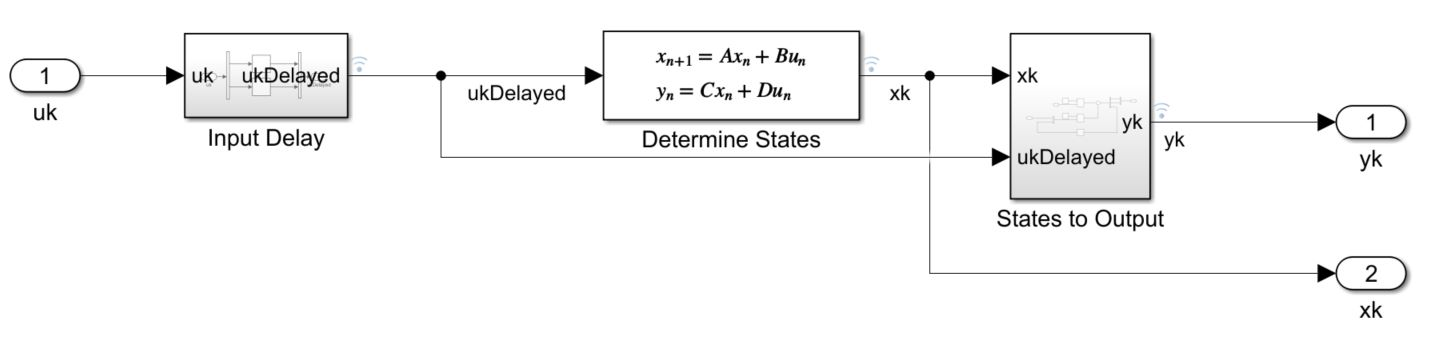
\includegraphics[width=17cm]{DiscretePlant.jpg}
	\centering
	\caption{Simulink Discrete Plant Implementation}
	\label{fig:DiscretePlant}
\end{figure}

\begin{figure}[H]
	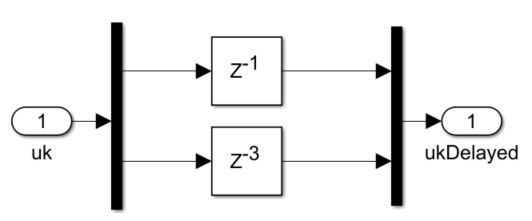
\includegraphics[width=8cm]{InputDelay.jpg}
	\centering
	\caption{Simulink Input Delay Block}
	\label{fig:InputDelay}
\end{figure}

\begin{figure}[H]
	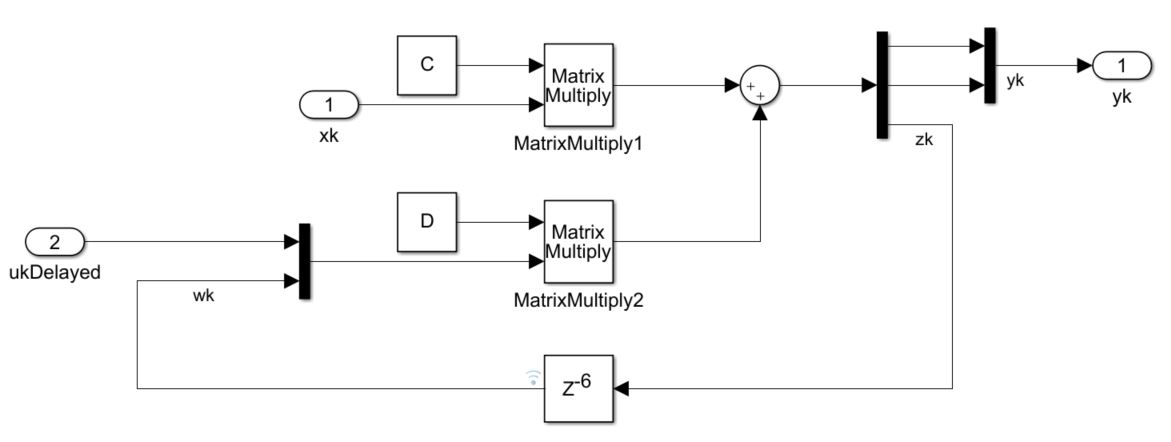
\includegraphics[width=17cm]{StatesToOutput.jpg}
	\centering
	\caption{Simulink States to Output Block}
	\label{fig:StatesToOutput}
\end{figure}

\section{Prediction and Control Horizon}

\begin{problem}{5} Document the prediction horizon that will lead to 99\% of steady-state for the slowest model to a unit step. \end{problem}

By implementing MATLAB's step function on the plant in (\ref{eq1}), as seen in Section \ref{code:Setup}, a step response of each input variable to each output variable is generated, as seen in Figure \ref{fig:StepResponse}. It is found that for the response of output 1 to a step in input 2 reaches 99\% of it's steady state value ($-18.9$) after $ 99.7 \, s $, which is the slowest observed response.

The prediction horizon, $N_P$, is chosen to cover the longest plant dynamics and the control horizon. The chosen value for the control horizon and prediction horizon is given under \textbf{Problem 6}.

\begin{figure}[h!]
	%% This file was created by matlab2tikz.
%
%The latest updates can be retrieved from
%  http://www.mathworks.com/matlabcentral/fileexchange/22022-matlab2tikz-matlab2tikz
%where you can also make suggestions and rate matlab2tikz.
%
\definecolor{mycolor1}{rgb}{0.00000,0.44700,0.74100}%
%
\begin{tikzpicture}

\begin{axis}[%
width=2.115in,
height=1.595in,
at={(0.883in,2.243in)},
scale only axis,
separate axis lines,
every outer x axis line/.append style={white!40!black},
every x tick label/.append style={font=\color{white!40!black}},
every x tick/.append style={white!40!black},
xmin=0,
xmax=140,
xtick={0,50,100},
xticklabels={\empty},
every outer y axis line/.append style={white!40!black},
every y tick label/.append style={font=\color{white!40!black}},
every y tick/.append style={white!40!black},
ymin=-20,
ymax=15,
ylabel style={font=\color{white!40!black}},
ylabel={To: Out(1)},
axis background/.style={fill=white},
title style={font=\color{white!40!black}},
title={From: In(1)},
legend style={legend cell align=left, align=left, draw=white!15!black}
]
\addplot [color=mycolor1, forget plot]
  table[row sep=crcr]{%
0	0\\
0.96708573905299	0\\
1.93417147810598	0.696353642523119\\
2.90125721715897	1.37735905786414\\
3.86834295621196	2.02004805499311\\
4.83542869526495	2.62657648740478\\
5.80251443431794	3.19897891060968\\
6.76960017337093	3.73917540690265\\
7.73668591242392	4.24897802613918\\
8.70377165147691	4.73009686412489\\
9.6708573905299	5.18414579900752\\
10.6379431295829	5.61264790491379\\
11.6050288686359	6.01704056099075\\
12.5721146076889	6.39868027298963\\
13.5392003467419	6.75884722356568\\
14.5062860857948	7.09874956655778\\
15.4733718248478	7.41952747965263\\
16.4404575639008	7.72225698902784\\
17.4075433029538	8.00795357880353\\
18.3746290420068	8.27757559740988\\
19.3417147810598	8.5320274722973\\
20.3088005201128	8.77216274377247\\
21.2758862591658	8.99878692813728\\
22.2429719982188	9.21266021973461\\
23.2100577372718	9.414500040965\\
24.1771434763247	9.6049834488279\\
25.1442292153777	9.78474940606015\\
26.1113149544307	9.95440092448995\\
27.0784006934837	10.1145070877962\\
28.0454864325367	10.2656049604585\\
29.0125721715897	10.4082013893003\\
29.9796579106427	10.5427747036706\\
30.9467436496957	10.6697763199642\\
31.9138293887487	10.7896322558653\\
32.8809151278017	10.9027445593933\\
33.8480008668546	11.0094926575431\\
34.8150866059076	11.1102346290456\\
35.7821723449606	11.2053084055167\\
36.7492580840136	11.2950329050243\\
37.7163438230666	11.379709101876\\
38.6834295621196	11.459621036215\\
39.6505153011726	11.5350367668129\\
40.6176010402256	11.6062092702523\\
41.5846867792786	11.6733772895195\\
42.5517725183316	11.7367661348495\\
43.5188582573845	11.7965884395135\\
44.4859439964375	11.8530448730811\\
45.4530297354905	11.9063248145525\\
46.4201154745435	11.9566069876159\\
47.3872012135965	12.0040600601638\\
48.3542869526495	12.0488432100762\\
49.3213726917025	12.0911066591725\\
50.2884584307555	12.1309921771185\\
51.2555441698085	12.168633556983\\
52.2226299088615	12.204157064037\\
53.1897156479144	12.2376818593011\\
54.1568013869674	12.2693203992626\\
55.1238871260204	12.2991788131025\\
56.0909728650734	12.3273572586982\\
57.0580586041264	12.3539502585961\\
58.0251443431794	12.3790470170799\\
58.9922300822324	12.4027317194007\\
59.9593158212854	12.4250838141696\\
60.9264015603384	12.4461782798627\\
61.8934872993914	12.4660858763309\\
62.8605730384443	12.4848733821586\\
63.8276587774973	12.5026038186676\\
64.7947445165503	12.5193366613174\\
65.7618302556033	12.5351280392118\\
66.7289159946563	12.5500309233792\\
67.6960017337093	12.5640953044606\\
68.6630874727623	12.5773683603995\\
69.6301732118153	12.5898946146964\\
70.5972589508683	12.6017160857604\\
71.5643446899213	12.6128724278564\\
72.5314304289742	12.6234010641223\\
73.4985161680272	12.6333373121028\\
74.4656019070802	12.642714502219\\
75.4326876461332	12.6515640895731\\
76.3997733851862	12.6599157594622\\
77.3668591242392	12.6677975269554\\
78.3339448632922	12.6752358308686\\
79.3010306023452	12.6822556224512\\
80.2681163413982	12.6888804490835\\
81.2352020804511	12.6951325332645\\
82.2022878195041	12.701032847156\\
83.1693735585571	12.7066011829316\\
84.1364592976101	12.7118562191687\\
85.1035450366631	12.7168155835042\\
86.0706307757161	12.721495911765\\
87.0377165147691	12.7259129037718\\
88.0048022538221	12.7300813760031\\
88.9718879928751	12.7340153112957\\
89.9389737319281	12.7377279057495\\
90.906059470981	12.7412316129925\\
91.873145210034	12.7445381859558\\
92.840230949087	12.7476587162979\\
93.80731668814	12.7506036716109\\
94.774402427193	12.7533829305331\\
95.741488166246	12.7560058158866\\
96.708573905299	12.7584811259493\\
97.675659644352	12.760817163969\\
98.642745383405	12.7630217660151\\
99.609831122458	12.765102327265\\
100.576916861511	12.76706582681\\
101.544002600564	12.7689188510664\\
102.511088339617	12.7706676158695\\
103.47817407867	12.7723179873235\\
104.445259817723	12.7738755014794\\
105.412345556776	12.7753453829053\\
106.379431295829	12.7767325622113\\
107.346517034882	12.7780416925896\\
108.313602773935	12.7792771654229\\
109.280688512988	12.7804431250149\\
110.247774252041	12.7815434824922\\
111.214859991094	12.7825819289239\\
112.181945730147	12.7835619477032\\
113.1490314692	12.7844868262316\\
114.116117208253	12.785359666947\\
115.083202947306	12.78618339773\\
116.050288686359	12.7869607817257\\
117.017374425412	12.787694426612\\
117.984460164465	12.7883867933475\\
118.951545903518	12.789040204426\\
119.918631642571	12.7896568516674\\
120.885717381624	12.79023880357\\
121.852803120677	12.7907880122491\\
122.81988885973	12.7913063199854\\
123.786974598783	12.7917954654044\\
124.754060337836	12.7922570893089\\
125.721146076889	12.7926927401827\\
126.688231815942	12.7931038793848\\
127.655317554995	12.793491886052\\
128.622403294048	12.7938580617243\\
129.589489033101	12.7942036347114\\
130.556574772154	12.7945297642127\\
131.523660511207	12.794837544206\\
132.49074625026	12.7951280071168\\
133.457831989313	12.7954021272818\\
134.424917728366	12.7956608242172\\
135.392003467419	12.7959049657031\\
136.359089206472	12.7961353706943\\
137.326174945525	12.7963528120675\\
138.293260684578	12.7965580192142\\
139.260346423631	12.7967516804866\\
140.227432162684	12.7969344455075\\
141.194517901737	12.7971069273488\\
142.16160364079	12.7972697045883\\
143.128689379843	12.7974233232505\\
144.095775118895	12.7975682986379\\
145.062860857948	12.79770511706\\
146.029946597001	12.7978342374642\\
146.997032336054	12.7979560929755\\
147.964118075107	12.7980710923493\\
148.93120381416	12.7981796213427\\
149.898289553213	12.7982820440083\\
150.865375292266	12.7983787039155\\
151.832461031319	12.7984699253029\\
152.799546770372	12.798556014166\\
153.766632509425	12.7986372592837\\
154.733718248478	12.7987139331868\\
155.700803987531	12.7987862930723\\
156.667889726584	12.7988545816661\\
157.634975465637	12.7989190280375\\
158.60206120469	12.7989798483671\\
159.569146943743	12.7990372466722\\
160.536232682796	12.7990914154912\\
161.503318421849	12.7991425365297\\
162.470404160902	12.7991907812693\\
163.437489899955	12.7992363115435\\
164.404575639008	12.7992792800804\\
165.371661378061	12.7993198310147\\
166.338747117114	12.7993581003716\\
167.305832856167	12.7993942165229\\
168.27291859522	12.7994283006175\\
169.240004334273	12.7994604669882\\
170.207090073326	12.7994908235347\\
171.174175812379	12.7995194720857\\
172.141261551432	12.7995465087408\\
173.108347290485	12.7995720241924\\
174.075433029538	12.7995961040303\\
175.042518768591	12.7996188290286\\
176.009604507644	12.7996402754166\\
176.976690246697	12.7996605151346\\
177.94377598575	12.7996796160753\\
178.910861724803	12.7996976423115\\
179.877947463856	12.7997146543108\\
180.845033202909	12.7997307091387\\
181.812118941962	12.79974586065\\
182.779204681015	12.7997601596694\\
183.746290420068	12.7997736541618\\
184.713376159121	12.7997863893936\\
185.680461898174	12.7997984080841\\
186.647547637227	12.7998097505492\\
187.61463337628	12.7998204548363\\
188.581719115333	12.7998305568523\\
189.548804854386	12.7998400904836\\
190.515890593439	12.79984908771\\
191.482976332492	12.7998575787121\\
192.450062071545	12.7998655919723\\
1934171478105.98	12.8\\
};
\addlegendentry{G}

\addplot [color=black, dotted, forget plot]
  table[row sep=crcr]{%
-1e+99	12.8\\
-1e+96	12.8\\
-1e+93	12.8\\
-1e+90	12.8\\
-1e+87	12.8\\
-1e+84	12.8\\
-1e+81	12.8\\
-1e+78	12.8\\
-1e+75	12.8\\
-1e+72	12.8\\
-1e+69	12.8\\
-1e+66	12.8\\
-1e+63	12.8\\
-1e+60	12.8\\
-1e+57	12.8\\
-1e+54	12.8\\
-1e+51	12.8\\
-1e+48	12.8\\
-1e+45	12.8\\
-1e+42	12.8\\
-1e+39	12.8\\
-1e+36	12.8\\
-1e+33	12.8\\
-1e+30	12.8\\
-1e+27	12.8\\
-1e+24	12.8\\
-1e+21	12.8\\
-1e+18	12.8\\
-1e+15	12.8\\
-1000000000000	12.8\\
-1000000000	12.8\\
-1000000	12.8\\
-1000	12.8\\
-1	12.8\\
0	12.8\\
1	12.8\\
1000	12.8\\
1000000	12.8\\
1000000000	12.8\\
1000000000000	12.8\\
1e+15	12.8\\
1e+18	12.8\\
1e+21	12.8\\
1e+24	12.8\\
1e+27	12.8\\
1e+30	12.8\\
1e+33	12.8\\
1e+36	12.8\\
1e+39	12.8\\
1e+42	12.8\\
1e+45	12.8\\
1e+48	12.8\\
1e+51	12.8\\
1e+54	12.8\\
1e+57	12.8\\
1e+60	12.8\\
1e+63	12.8\\
1e+66	12.8\\
1e+69	12.8\\
1e+72	12.8\\
1e+75	12.8\\
1e+78	12.8\\
1e+81	12.8\\
1e+84	12.8\\
1e+87	12.8\\
1e+90	12.8\\
1e+93	12.8\\
1e+96	12.8\\
1e+99	12.8\\
};
\end{axis}

\begin{axis}[%
width=2.115in,
height=1.595in,
at={(0.883in,0.481in)},
scale only axis,
separate axis lines,
every outer x axis line/.append style={white!40!black},
every x tick label/.append style={font=\color{white!40!black}},
every x tick/.append style={white!40!black},
xmin=0,
xmax=140,
every outer y axis line/.append style={white!40!black},
every y tick label/.append style={font=\color{white!40!black}},
every y tick/.append style={white!40!black},
ymin=-20,
ymax=8,
ylabel style={font=\color{white!40!black}},
ylabel={To: Out(2)},
axis background/.style={fill=white},
legend style={legend cell align=left, align=left, draw=white!15!black}
]
\addplot [color=mycolor1, forget plot]
  table[row sep=crcr]{%
0	0\\
0.96708573905299	0\\
1.93417147810598	0\\
2.90125721715897	0\\
3.86834295621196	0\\
4.83542869526495	0\\
5.80251443431794	0\\
6.76960017337093	0\\
7.73668591242392	0.431326730706558\\
8.70377165147691	0.955055740672238\\
9.6708573905299	1.43431942334542\\
10.6379431295829	1.87289294736027\\
11.6050288686359	2.27423096424058\\
12.5721146076889	2.64149482075181\\
13.5392003467419	2.97757746088638\\
14.5062860857948	3.28512621363539\\
15.4733718248478	3.56656364604665\\
16.4404575639008	3.82410664582882\\
17.4075433029538	4.05978388381567\\
18.3746290420068	4.27545179384269\\
19.3417147810598	4.47280919590975\\
20.3088005201128	4.65341067781672\\
21.2758862591658	4.81867884067949\\
22.2429719982188	4.96991550478452\\
23.2100577372718	5.10831196405062\\
24.1771434763247	5.23495836987248\\
25.1442292153777	5.35085231826286\\
26.1113149544307	5.45690670793425\\
27.0784006934837	5.55395693121842\\
28.0454864325367	5.64276745446683\\
29.0125721715897	5.72403783976581\\
29.9796579106427	5.79840825539967\\
30.9467436496957	5.86646451846777\\
31.9138293887487	5.92874270937633\\
32.8809151278017	5.98573339455341\\
33.8480008668546	6.03788549064949\\
34.8150866059076	6.08560980066198\\
35.7821723449606	6.12928224983778\\
36.7492580840136	6.16924684684325\\
37.7163438230666	6.20581839352661\\
38.6834295621196	6.23928496461778\\
39.6505153011726	6.26991017689817\\
40.6176010402256	6.29793526571482\\
41.5846867792786	6.32358098519557\\
42.5517725183316	6.34704934713328\\
43.5188582573845	6.36852521223631\\
44.4859439964375	6.38817774627973\\
45.4530297354905	6.40616175262706\\
46.4201154745435	6.42261889161924\\
47.3872012135965	6.43767879643562\\
48.3542869526495	6.45146009421684\\
49.3213726917025	6.464071340493\\
50.2884584307555	6.47561187427746\\
51.2555441698085	6.48617260056206\\
52.2226299088615	6.49583670637738\\
53.1897156479144	6.50468031605846\\
54.1568013869674	6.51277309087755\\
55.1238871260204	6.52017877776722\\
56.0909728650734	6.52695571145608\\
57.0580586041264	6.53315727397248\\
58.0251443431794	6.53883231513571\\
58.9922300822324	6.54402553734693\\
59.9593158212854	6.54877784771075\\
60.9264015603384	6.55312668026122\\
61.8934872993914	6.55710629083045\\
62.8605730384443	6.56074802688234\\
63.8276587774973	6.56408057443717\\
64.7947445165503	6.56713018403186\\
65.7618302556033	6.56992087749596\\
66.7289159946563	6.57247463717198\\
67.6960017337093	6.57481157907075\\
68.6630874727623	6.57695011132558\\
69.6301732118153	6.57890707919343\\
70.5972589508683	6.58069789774534\\
71.5643446899213	6.58233667329119\\
72.5314304289742	6.5838363144954\\
73.4985161680272	6.58520863405864\\
74.4656019070802	6.58646444176677\\
75.4326876461332	6.58761362963965\\
76.3997733851862	6.58866524985079\\
77.3668591242392	6.58962758603147\\
78.3339448632922	6.59050821852107\\
79.3010306023452	6.59131408407753\\
80.2681163413982	6.5920515305183\\
81.2352020804511	6.59272636672224\\
82.2022878195041	6.59334390838625\\
83.1693735585571	6.59390901989709\\
84.1364592976101	6.59442615264829\\
85.1035450366631	6.59489938010382\\
86.0706307757161	6.59533242988484\\
87.0377165147691	6.59572871313225\\
88.0048022538221	6.5960913513763\\
88.9718879928751	6.59642320112496\\
89.9389737319281	6.59672687636466\\
90.906059470981	6.59700476915071\\
91.873145210034	6.59725906844958\\
92.840230949087	6.5974917773814\\
93.80731668814	6.59770472899863\\
94.774402427193	6.59789960072495\\
95.741488166246	6.59807792756848\\
96.708573905299	6.59824111421295\\
97.675659644352	6.59839044608249\\
98.642745383405	6.59852709946692\\
99.609831122458	6.59865215078741\\
100.576916861511	6.59876658507544\\
101.544002600564	6.59887130373197\\
102.511088339617	6.59896713162772\\
103.47817407867	6.59905482360077\\
104.445259817723	6.59913507040234\\
105.412345556776	6.59920850413794\\
106.379431295829	6.59927570324643\\
107.346517034882	6.59933719705638\\
108.313602773935	6.59939346995564\\
109.280688512988	6.59944496520685\\
110.247774252041	6.59949208843903\\
111.214859991094	6.59953521084273\\
112.181945730147	6.59957467209388\\
113.1490314692	6.59961078302948\\
114.116117208253	6.59964382809602\\
115.083202947306	6.59967406759007\\
116.050288686359	6.59970173970868\\
117.017374425412	6.59972706242562\\
117.984460164465	6.59975023520838\\
118.951545903518	6.5997714405894\\
119.918631642571	6.59979084560383\\
120.885717381624	6.59980860310533\\
121.852803120677	6.59982485297006\\
122.81988885973	6.59983972319848\\
123.786974598783	6.59985333092366\\
124.754060337836	6.5998657833339\\
125.721146076889	6.59987717851704\\
126.688231815942	6.59988760623316\\
127.655317554995	6.59989714862155\\
128.622403294048	6.5999058808478\\
129.589489033101	6.59991387169579\\
130.556574772154	6.59992118410958\\
131.523660511207	6.59992787568919\\
132.49074625026	6.59993399914431\\
133.457831989313	6.5999396027095\\
134.424917728366	6.59994473052415\\
135.392003467419	6.59994942298014\\
136.359089206472	6.59995371704004\\
137.326174945525	6.59995764652824\\
138.293260684578	6.59996124239738\\
139.260346423631	6.59996453297218\\
140.227432162684	6.59996754417258\\
141.194517901737	6.59997029971783\\
142.16160364079	6.59997282131343\\
143.128689379843	6.59997512882203\\
144.095775118895	6.59997724041991\\
145.062860857948	6.59997917274017\\
146.029946597001	6.59998094100373\\
146.997032336054	6.59998255913924\\
147.964118075107	6.59998403989277\\
148.93120381416	6.59998539492826\\
149.898289553213	6.59998663491933\\
150.865375292266	6.59998776963341\\
151.832461031319	6.59998880800869\\
152.799546770372	6.59998975822444\\
153.766632509425	6.59999062776555\\
154.733718248478	6.59999142348139\\
155.700803987531	6.59999215163985\\
156.667889726584	6.59999281797663\\
157.634975465637	6.59999342774048\\
158.60206120469	6.59999398573453\\
159.569146943743	6.5999944963541\\
160.536232682796	6.59999496362136\\
161.503318421849	6.59999539121696\\
162.470404160902	6.59999578250911\\
163.437489899955	6.59999614058\\
164.404575639008	6.59999646825017\\
165.371661378061	6.59999676810068\\
166.338747117114	6.59999704249346\\
167.305832856167	6.59999729358992\\
168.27291859522	6.59999752336793\\
169.240004334273	6.59999773363746\\
170.207090073326	6.59999792605482\\
171.174175812379	6.59999810213567\\
172.141261551432	6.59999826326701\\
173.108347290485	6.59999841071808\\
174.075433029538	6.59999854565034\\
175.042518768591	6.59999866912667\\
176.009604507644	6.59999878211968\\
176.976690246697	6.59999888551943\\
177.94377598575	6.59999898014039\\
178.910861724803	6.5999990667279\\
179.877947463856	6.59999914596401\\
180.845033202909	6.59999921847286\\
181.812118941962	6.59999928482561\\
182.779204681015	6.59999934554492\\
183.746290420068	6.59999940110907\\
184.713376159121	6.59999945195575\\
185.680461898174	6.59999949848548\\
186.647547637227	6.59999954106476\\
187.61463337628	6.59999958002901\\
188.581719115333	6.59999961568514\\
189.548804854386	6.59999964831401\\
190.515890593439	6.59999967817264\\
191.482976332492	6.59999970549623\\
192.450062071545	6.59999973050002\\
1934171478105.98	6.6\\
};
\addlegendentry{G}

\addplot [color=black, dotted, forget plot]
  table[row sep=crcr]{%
-1e+99	6.6\\
-1e+96	6.6\\
-1e+93	6.6\\
-1e+90	6.6\\
-1e+87	6.6\\
-1e+84	6.6\\
-1e+81	6.6\\
-1e+78	6.6\\
-1e+75	6.6\\
-1e+72	6.6\\
-1e+69	6.6\\
-1e+66	6.6\\
-1e+63	6.6\\
-1e+60	6.6\\
-1e+57	6.6\\
-1e+54	6.6\\
-1e+51	6.6\\
-1e+48	6.6\\
-1e+45	6.6\\
-1e+42	6.6\\
-1e+39	6.6\\
-1e+36	6.6\\
-1e+33	6.6\\
-1e+30	6.6\\
-1e+27	6.6\\
-1e+24	6.6\\
-1e+21	6.6\\
-1e+18	6.6\\
-1e+15	6.6\\
-1000000000000	6.6\\
-1000000000	6.6\\
-1000000	6.6\\
-1000	6.6\\
-1	6.6\\
0	6.6\\
1	6.6\\
1000	6.6\\
1000000	6.6\\
1000000000	6.6\\
1000000000000	6.6\\
1e+15	6.6\\
1e+18	6.6\\
1e+21	6.6\\
1e+24	6.6\\
1e+27	6.6\\
1e+30	6.6\\
1e+33	6.6\\
1e+36	6.6\\
1e+39	6.6\\
1e+42	6.6\\
1e+45	6.6\\
1e+48	6.6\\
1e+51	6.6\\
1e+54	6.6\\
1e+57	6.6\\
1e+60	6.6\\
1e+63	6.6\\
1e+66	6.6\\
1e+69	6.6\\
1e+72	6.6\\
1e+75	6.6\\
1e+78	6.6\\
1e+81	6.6\\
1e+84	6.6\\
1e+87	6.6\\
1e+90	6.6\\
1e+93	6.6\\
1e+96	6.6\\
1e+99	6.6\\
};
\end{axis}

\begin{axis}[%
width=2.115in,
height=1.595in,
at={(3.165in,2.243in)},
scale only axis,
separate axis lines,
every outer x axis line/.append style={white!40!black},
every x tick label/.append style={font=\color{white!40!black}},
every x tick/.append style={white!40!black},
xmin=0,
xmax=140,
xtick={0,50,100},
xticklabels={\empty},
every outer y axis line/.append style={white!40!black},
every y tick label/.append style={font=\color{white!40!black}},
every y tick/.append style={white!40!black},
ymin=-20,
ymax=15,
ytick={-20,-10,0,10},
yticklabels={\empty},
axis background/.style={fill=white},
title style={font=\color{white!40!black}},
title={From: In(2)},
legend style={legend cell align=left, align=left, draw=white!15!black}
]
\addplot [color=mycolor1, forget plot]
  table[row sep=crcr]{%
0	0\\
0.96708573905299	0\\
1.93417147810598	0\\
2.90125721715897	0\\
3.86834295621196	-0.765571520067246\\
4.83542869526495	-1.58175524992452\\
5.80251443431794	-2.36120466076971\\
6.76960017337093	-3.1055730693058\\
7.73668591242392	-3.8164393807265\\
8.70377165147691	-4.49531143778581\\
9.6708573905299	-5.14362921913472\\
10.6379431295829	-5.76276789370893\\
11.6050288686359	-6.35404073764656\\
12.5721146076889	-6.91870191992293\\
13.5392003467419	-7.45794916261107\\
14.5062860857948	-7.97292628141087\\
15.4733718248478	-8.46472561183545\\
16.4404575639008	-8.93439032620134\\
17.4075433029538	-9.38291664633674\\
18.3746290420068	-9.81125595670161\\
19.3417147810598	-10.2203168224017\\
20.3088005201128	-10.6109669163769\\
21.2758862591658	-10.9840348598518\\
22.2429719982188	-11.3403119799527\\
23.2100577372718	-11.6805539882182\\
24.1771434763247	-12.0054825835649\\
25.1442292153777	-12.3157869831074\\
26.1113149544307	-12.6121253840804\\
27.0784006934837	-12.8951263599631\\
28.0454864325367	-13.165390193768\\
29.0125721715897	-13.4234901513214\\
29.9796579106427	-13.6699736972375\\
30.9467436496957	-13.9053636561636\\
31.9138293887487	-14.130159321762\\
32.8809151278017	-14.3448375157783\\
33.8480008668546	-14.5498535994443\\
34.8150866059076	-14.7456424393606\\
35.7821723449606	-14.9326193299064\\
36.7492580840136	-15.1111808741351\\
37.7163438230666	-15.281705825022\\
38.6834295621196	-15.4445558888507\\
39.6505153011726	-15.6000764924403\\
40.6176010402256	-15.748597515842\\
41.5846867792786	-15.8904339920589\\
42.5517725183316	-16.0258867752735\\
43.5188582573845	-16.1552431789994\\
44.4859439964375	-16.2787775855121\\
45.4530297354905	-16.3967520278503\\
46.4201154745435	-16.5094167456234\\
47.3872012135965	-16.6170107158028\\
48.3542869526495	-16.7197621596249\\
49.3213726917025	-16.8178890266779\\
50.2884584307555	-16.9115994572031\\
51.2555441698085	-17.0010922235876\\
52.2226299088615	-17.0865571519873\\
53.1897156479144	-17.1681755249739\\
54.1568013869674	-17.2461204660592\\
55.1238871260204	-17.3205573069136\\
56.0909728650734	-17.3916439380565\\
57.0580586041264	-17.4595311437631\\
58.0251443431794	-17.5243629218987\\
58.9922300822324	-17.5862767893568\\
59.9593158212854	-17.6454040737512\\
60.9264015603384	-17.7018701919795\\
61.8934872993914	-17.7557949162489\\
62.8605730384443	-17.8072926281294\\
63.8276587774973	-17.8564725611724\\
64.7947445165503	-17.9034390326095\\
65.7618302556033	-17.9482916646235\\
66.7289159946563	-17.9911255956604\\
67.6960017337093	-18.0320316822309\\
68.6630874727623	-18.0710966916288\\
69.6301732118153	-18.1084034859767\\
70.5972589508683	-18.1440311979872\\
71.5643446899213	-18.1780553988141\\
72.5314304289742	-18.2105482583491\\
73.4985161680272	-18.2415786983037\\
74.4656019070802	-18.2712125384013\\
75.4326876461332	-18.2995126359899\\
76.3997733851862	-18.3265390193707\\
77.3668591242392	-18.3523490151263\\
78.3339448632922	-18.3769973697182\\
79.3010306023452	-18.400536365611\\
80.2681163413982	-18.4230159321711\\
81.2352020804511	-18.444483751573\\
82.2022878195041	-18.4649853599398\\
83.1693735585571	-18.4845642439316\\
84.1364592976101	-18.5032619329864\\
85.1035450366631	-18.5211180874095\\
86.0706307757161	-18.5381705824983\\
87.0377165147691	-18.5544555888814\\
88.0048022538221	-18.5700076492405\\
88.9718879928751	-18.5848597515808\\
89.9389737319281	-18.5990433992027\\
90.906059470981	-18.6125886775243\\
91.873145210034	-18.625524317897\\
92.840230949087	-18.6378777585484\\
93.80731668814	-18.6496752027824\\
94.774402427193	-18.6609416745598\\
95.741488166246	-18.6717010715779\\
96.708573905299	-18.6819762159602\\
97.675659644352	-18.6917889026656\\
98.642745383405	-18.7011599457182\\
99.609831122458	-18.7101092223567\\
100.576916861511	-18.7186557151968\\
101.544002600564	-18.7268175524956\\
102.511088339617	-18.7346120466042\\
103.47817407867	-18.7420557306897\\
104.445259817723	-18.7491643938041\\
105.412345556776	-18.7559531143748\\
106.379431295829	-18.7624362921884\\
107.346517034882	-18.7686276789343\\
108.313602773935	-18.7745404073738\\
109.280688512988	-18.7801870191967\\
110.247774252041	-18.7855794916237\\
111.214859991094	-18.7907292628118\\
112.181945730147	-18.7956472561161\\
113.1490314692	-18.8003439032599\\
114.116117208253	-18.8048291664614\\
115.083202947306	-18.8091125595651\\
116.050288686359	-18.8132031682222\\
117.017374425412	-18.817109669162\\
117.984460164465	-18.8208403485968\\
118.951545903518	-18.8244031197979\\
119.918631642571	-18.8278055398807\\
120.885717381624	-18.8310548258342\\
121.852803120677	-18.8341578698297\\
122.81988885973	-18.8371212538395\\
123.786974598783	-18.8399512635984\\
124.754060337836	-18.8426539019365\\
125.721146076889	-18.8452349015121\\
126.688231815942	-18.8476997369713\\
127.655317554995	-18.8500536365606\\
128.622403294048	-18.8523015932166\\
129.589489033101	-18.8544483751568\\
130.556574772154	-18.8564985359935\\
131.523660511207	-18.8584564243927\\
132.49074625026	-18.8603261932982\\
133.457831989313	-18.8621118087406\\
134.424917728366	-18.8638170582495\\
135.392003467419	-18.8654455588878\\
136.359089206472	-18.8670007649237\\
137.326174945525	-18.8684859751578\\
138.293260684578	-18.86990433992\\
139.260346423631	-18.8712588677522\\
140.227432162684	-18.8725524317894\\
141.194517901737	-18.8737877758546\\
142.16160364079	-18.874967520278\\
143.128689379843	-18.8760941674558\\
144.095775118895	-18.8771701071576\\
145.062860857948	-18.8781976215958\\
146.029946597001	-18.8791788902664\\
146.997032336054	-18.8801159945716\\
147.964118075107	-18.8810109222355\\
148.93120381416	-18.8818655715195\\
149.898289553213	-18.8826817552494\\
150.865375292266	-18.8834612046603\\
151.832461031319	-18.8842055730688\\
152.799546770372	-18.8849164393803\\
153.766632509425	-18.8855953114374\\
154.733718248478	-18.8862436292187\\
155.700803987531	-18.8868627678933\\
156.667889726584	-18.8874540407373\\
157.634975465637	-18.8880187019196\\
158.60206120469	-18.8885579491623\\
159.569146943743	-18.8890729262811\\
160.536232682796	-18.8895647256115\\
161.503318421849	-18.8900343903259\\
162.470404160902	-18.8904829166461\\
163.437489899955	-18.8909112559564\\
164.404575639008	-18.8913203168222\\
165.371661378061	-18.8917109669161\\
166.338747117114	-18.8920840348596\\
167.305832856167	-18.8924403119797\\
168.27291859522	-18.892780553988\\
169.240004334273	-18.8931054825834\\
170.207090073326	-18.8934157869829\\
171.174175812379	-18.8937121253839\\
172.141261551432	-18.8939951263598\\
173.108347290485	-18.8942653901936\\
174.075433029538	-18.8945234901512\\
175.042518768591	-18.8947699736971\\
176.009604507644	-18.895005363656\\
176.976690246697	-18.8952301593216\\
177.94377598575	-18.8954448375157\\
178.910861724803	-18.8956498535993\\
179.877947463856	-18.8958456424393\\
180.845033202909	-18.8960326193298\\
181.812118941962	-18.896211180874\\
182.779204681015	-18.8963817058249\\
183.746290420068	-18.8965445558888\\
184.713376159121	-18.8967000764924\\
185.680461898174	-18.8968485975158\\
186.647547637227	-18.896990433992\\
187.61463337628	-18.8971258867752\\
188.581719115333	-18.8972552431789\\
189.548804854386	-18.8973787775855\\
190.515890593439	-18.8974967520278\\
191.482976332492	-18.8976094167456\\
192.450062071545	-18.8977170107158\\
1934171478105.98	-18.9\\
};
\addlegendentry{G}

\addplot [color=black, dotted, forget plot]
  table[row sep=crcr]{%
-1e+99	-18.9\\
-1e+96	-18.9\\
-1e+93	-18.9\\
-1e+90	-18.9\\
-1e+87	-18.9\\
-1e+84	-18.9\\
-1e+81	-18.9\\
-1e+78	-18.9\\
-1e+75	-18.9\\
-1e+72	-18.9\\
-1e+69	-18.9\\
-1e+66	-18.9\\
-1e+63	-18.9\\
-1e+60	-18.9\\
-1e+57	-18.9\\
-1e+54	-18.9\\
-1e+51	-18.9\\
-1e+48	-18.9\\
-1e+45	-18.9\\
-1e+42	-18.9\\
-1e+39	-18.9\\
-1e+36	-18.9\\
-1e+33	-18.9\\
-1e+30	-18.9\\
-1e+27	-18.9\\
-1e+24	-18.9\\
-1e+21	-18.9\\
-1e+18	-18.9\\
-1e+15	-18.9\\
-1000000000000	-18.9\\
-1000000000	-18.9\\
-1000000	-18.9\\
-1000	-18.9\\
-1	-18.9\\
0	-18.9\\
1	-18.9\\
1000	-18.9\\
1000000	-18.9\\
1000000000	-18.9\\
1000000000000	-18.9\\
1e+15	-18.9\\
1e+18	-18.9\\
1e+21	-18.9\\
1e+24	-18.9\\
1e+27	-18.9\\
1e+30	-18.9\\
1e+33	-18.9\\
1e+36	-18.9\\
1e+39	-18.9\\
1e+42	-18.9\\
1e+45	-18.9\\
1e+48	-18.9\\
1e+51	-18.9\\
1e+54	-18.9\\
1e+57	-18.9\\
1e+60	-18.9\\
1e+63	-18.9\\
1e+66	-18.9\\
1e+69	-18.9\\
1e+72	-18.9\\
1e+75	-18.9\\
1e+78	-18.9\\
1e+81	-18.9\\
1e+84	-18.9\\
1e+87	-18.9\\
1e+90	-18.9\\
1e+93	-18.9\\
1e+96	-18.9\\
1e+99	-18.9\\
};
\end{axis}

\begin{axis}[%
width=2.115in,
height=1.595in,
at={(3.165in,0.481in)},
scale only axis,
separate axis lines,
every outer x axis line/.append style={white!40!black},
every x tick label/.append style={font=\color{white!40!black}},
every x tick/.append style={white!40!black},
xmin=0,
xmax=140,
every outer y axis line/.append style={white!40!black},
every y tick label/.append style={font=\color{white!40!black}},
every y tick/.append style={white!40!black},
ymin=-20,
ymax=8,
ytick={-20,-15,-10,-5,0,5},
yticklabels={\empty},
axis background/.style={fill=white},
legend style={legend cell align=left, align=left, draw=white!15!black}
]
\addplot [color=mycolor1, forget plot]
  table[row sep=crcr]{%
0	0\\
0.96708573905299	0\\
1.93417147810598	0\\
2.90125721715897	0\\
3.86834295621196	-1.13527741327679\\
4.83542869526495	-2.32163018003838\\
5.80251443431794	-3.43092550010074\\
6.76960017337093	-4.46816850369001\\
7.73668591242392	-5.43803922164672\\
8.70377165147691	-6.34491370168162\\
9.6708573905299	-7.19288375306251\\
10.6379431295829	-7.98577540881982\\
11.6050288686359	-8.72716618877221\\
12.5721146076889	-9.42040124126301\\
13.5392003467419	-10.0686084364385\\
14.5062860857948	-10.6747124791692\\
15.4733718248478	-11.241448105291\\
16.4404575639008	-11.7713724207083\\
17.4075433029538	-12.2668764390319\\
18.3746290420068	-12.7301958698103\\
19.3417147810598	-13.1634212060309\\
20.3088005201128	-13.5685071564044\\
21.2758862591658	-13.9472814649931\\
22.2429719982188	-14.3014531579746\\
23.2100577372718	-14.6326202547526\\
24.1771434763247	-14.9422769782053\\
25.1442292153777	-15.2318204966055\\
26.1113149544307	-15.5025572276307\\
27.0784006934837	-15.7557087329077\\
28.0454864325367	-15.9924172296873\\
29.0125721715897	-16.2137507445181\\
29.9796579106427	-16.4207079321724\\
30.9467436496957	-16.6142225815669\\
31.9138293887487	-16.7951678290103\\
32.8809151278017	-16.9643600977858\\
33.8480008668546	-17.1225627818456\\
34.8150866059076	-17.2704896902372\\
35.7821723449606	-17.4088082678032\\
36.7492580840136	-17.5381426066867\\
37.7163438230666	-17.6590762622287\\
38.6834295621196	-17.7721548859647\\
39.6505153011726	-17.8778886875993\\
40.6176010402256	-17.9767547370677\\
41.5846867792786	-18.0691991170709\\
42.5517725183316	-18.1556389357966\\
43.5188582573845	-18.2364642089076\\
44.4859439964375	-18.3120396192887\\
45.4530297354905	-18.3827061624927\\
46.4201154745435	-18.4487826853091\\
47.3872012135965	-18.5105673243977\\
48.3542869526495	-18.5683388514789\\
49.3213726917025	-18.6223579311485\\
50.2884584307555	-18.6728682969946\\
51.2555441698085	-18.7200978513207\\
52.2226299088615	-18.7642596934392\\
53.1897156479144	-18.8055530811733\\
54.1568013869674	-18.8441643299068\\
55.1238871260204	-18.8802676532367\\
56.0909728650734	-18.9140259490241\\
57.0580586041264	-18.9455915343875\\
58.0251443431794	-18.9751068329561\\
58.9922300822324	-19.0027050174841\\
59.9593158212854	-19.0285106107248\\
60.9264015603384	-19.0526400472764\\
61.8934872993914	-19.0752021989335\\
62.8605730384443	-19.0962988659156\\
63.8276587774973	-19.1160252361892\\
64.7947445165503	-19.1344703149544\\
65.7618302556033	-19.1517173262362\\
66.7289159946563	-19.1678440883899\\
67.6960017337093	-19.1829233652171\\
68.6630874727623	-19.1970231942757\\
69.6301732118153	-19.2102071938637\\
70.5972589508683	-19.2225348500656\\
71.5643446899213	-19.234061785152\\
72.5314304289742	-19.2448400085475\\
73.4985161680272	-19.2549181514964\\
74.4656019070802	-19.2643416864864\\
75.4326876461332	-19.2731531324203\\
76.3997733851862	-19.2813922464607\\
77.3668591242392	-19.2890962034139\\
78.3339448632922	-19.2962997634625\\
79.3010306023452	-19.3030354290028\\
80.2681163413982	-19.3093335912954\\
81.2352020804511	-19.3152226675903\\
82.2022878195041	-19.3207292293454\\
83.1693735585571	-19.3258781221163\\
84.1364592976101	-19.3306925776596\\
85.1035450366631	-19.3351943187543\\
86.0706307757161	-19.3394036572144\\
87.0377165147691	-19.3433395855362\\
88.0048022538221	-19.3470198625919\\
88.9718879928751	-19.3504610937576\\
89.9389737319281	-19.3536788058364\\
90.906059470981	-19.3566875171154\\
91.873145210034	-19.3595008028723\\
92.840230949087	-19.3621313566261\\
93.80731668814	-19.3645910474113\\
94.774402427193	-19.3668909733298\\
95.741488166246	-19.3690415116262\\
96.708573905299	-19.3710523655093\\
97.675659644352	-19.3729326079332\\
98.642745383405	-19.3746907225345\\
99.609831122458	-19.3763346419098\\
100.576916861511	-19.3778717834083\\
101.544002600564	-19.3793090825982\\
102.511088339617	-19.3806530245601\\
103.47817407867	-19.3819096731477\\
104.445259817723	-19.3830846983478\\
105.412345556776	-19.3841834018633\\
106.379431295829	-19.3852107410343\\
107.346517034882	-19.3861713512056\\
108.313602773935	-19.3870695666414\\
109.280688512988	-19.3879094400814\\
110.247774252041	-19.3886947610269\\
111.214859991094	-19.3894290728387\\
112.181945730147	-19.3901156887249\\
113.1490314692	-19.39075770669\\
114.116117208253	-19.3913580235132\\
115.083202947306	-19.3919193478184\\
116.050288686359	-19.3924442122957\\
117.017374425412	-19.3929349851287\\
117.984460164465	-19.3933938806799\\
118.951545903518	-19.3938229694819\\
119.918631642571	-19.3942241875793\\
120.885717381624	-19.3945993452644\\
121.852803120677	-19.3949501352454\\
122.81988885973	-19.3952781402832\\
123.786974598783	-19.3955848403337\\
124.754060337836	-19.3958716192246\\
125.721146076889	-19.3961397708996\\
126.688231815942	-19.3963905052566\\
127.655317554995	-19.3966249536067\\
128.622403294048	-19.3968441737787\\
129.589489033101	-19.3970491548919\\
130.556574772154	-19.3972408218194\\
131.523660511207	-19.3974200393603\\
132.49074625026	-19.3975876161428\\
133.457831989313	-19.3977443082715\\
134.424917728366	-19.3978908227401\\
135.392003467419	-19.3980278206203\\
136.359089206472	-19.3981559200455\\
137.326174945525	-19.3982756989989\\
138.293260684578	-19.3983876979222\\
139.260346423631	-19.3984924221534\\
140.227432162684	-19.3985903442073\\
141.194517901737	-19.3986819059073\\
142.16160364079	-19.3987675203789\\
143.128689379843	-19.3988475739139\\
144.095775118895	-19.398922427713\\
145.062860857948	-19.398992419516\\
146.029946597001	-19.3990578651251\\
146.997032336054	-19.3991190598303\\
147.964118075107	-19.3991762797417\\
148.93120381416	-19.3992297830349\\
149.898289553213	-19.3992798111163\\
150.865375292266	-19.399326589712\\
151.832461031319	-19.3993703298868\\
152.799546770372	-19.3994112289959\\
153.766632509425	-19.3994494715756\\
154.733718248478	-19.3994852301762\\
155.700803987531	-19.3995186661401\\
156.667889726584	-19.39954993033\\
157.634975465637	-19.3995791638098\\
158.60206120469	-19.3996064984806\\
159.569146943743	-19.3996320576761\\
160.536232682796	-19.3996559567193\\
161.503318421849	-19.3996783034424\\
162.470404160902	-19.3996991986736\\
163.437489899955	-19.399718736692\\
164.404575639008	-19.3997370056529\\
165.371661378061	-19.3997540879858\\
166.338747117114	-19.399770060766\\
167.305832856167	-19.3997849960624\\
168.27291859522	-19.3997989612631\\
169.240004334273	-19.3998120193789\\
170.207090073326	-19.3998242293278\\
171.174175812379	-19.3998356462011\\
172.141261551432	-19.3998463215115\\
173.108347290485	-19.3998563034261\\
174.075433029538	-19.399865636983\\
175.042518768591	-19.3998743642953\\
176.009604507644	-19.3998825247404\\
176.976690246697	-19.3998901551382\\
177.94377598575	-19.399897289917\\
178.910861724803	-19.3999039612689\\
179.877947463856	-19.3999101992949\\
180.845033202909	-19.3999160321409\\
181.812118941962	-19.3999214861248\\
182.779204681015	-19.3999265858547\\
183.746290420068	-19.3999313543408\\
184.713376159121	-19.3999358130982\\
185.680461898174	-19.3999399822449\\
186.647547637227	-19.3999438805921\\
187.61463337628	-19.399947525729\\
188.581719115333	-19.3999509341026\\
189.548804854386	-19.3999541210912\\
190.515890593439	-19.3999571010746\\
191.482976332492	-19.3999598874985\\
192.450062071545	-19.3999624929351\\
1934171478105.98	-19.4\\
};
\addlegendentry{G}

\addplot [color=black, dotted, forget plot]
  table[row sep=crcr]{%
-1e+99	-19.4\\
-1e+96	-19.4\\
-1e+93	-19.4\\
-1e+90	-19.4\\
-1e+87	-19.4\\
-1e+84	-19.4\\
-1e+81	-19.4\\
-1e+78	-19.4\\
-1e+75	-19.4\\
-1e+72	-19.4\\
-1e+69	-19.4\\
-1e+66	-19.4\\
-1e+63	-19.4\\
-1e+60	-19.4\\
-1e+57	-19.4\\
-1e+54	-19.4\\
-1e+51	-19.4\\
-1e+48	-19.4\\
-1e+45	-19.4\\
-1e+42	-19.4\\
-1e+39	-19.4\\
-1e+36	-19.4\\
-1e+33	-19.4\\
-1e+30	-19.4\\
-1e+27	-19.4\\
-1e+24	-19.4\\
-1e+21	-19.4\\
-1e+18	-19.4\\
-1e+15	-19.4\\
-1000000000000	-19.4\\
-1000000000	-19.4\\
-1000000	-19.4\\
-1000	-19.4\\
-1	-19.4\\
0	-19.4\\
1	-19.4\\
1000	-19.4\\
1000000	-19.4\\
1000000000	-19.4\\
1000000000000	-19.4\\
1e+15	-19.4\\
1e+18	-19.4\\
1e+21	-19.4\\
1e+24	-19.4\\
1e+27	-19.4\\
1e+30	-19.4\\
1e+33	-19.4\\
1e+36	-19.4\\
1e+39	-19.4\\
1e+42	-19.4\\
1e+45	-19.4\\
1e+48	-19.4\\
1e+51	-19.4\\
1e+54	-19.4\\
1e+57	-19.4\\
1e+60	-19.4\\
1e+63	-19.4\\
1e+66	-19.4\\
1e+69	-19.4\\
1e+72	-19.4\\
1e+75	-19.4\\
1e+78	-19.4\\
1e+81	-19.4\\
1e+84	-19.4\\
1e+87	-19.4\\
1e+90	-19.4\\
1e+93	-19.4\\
1e+96	-19.4\\
1e+99	-19.4\\
};
\end{axis}

\begin{axis}[%
width=4.521in,
height=3.566in,
at={(0.758in,0.481in)},
scale only axis,
xmin=0,
xmax=1,
xtick={\empty},
xlabel={Time (seconds)},
ymin=0,
ymax=1,
ytick={\empty},
ylabel={Amplitude},
axis line style={draw=none},
ticks=none,
title style={font=\bfseries},
title={Step Response},
axis x line*=bottom,
axis y line*=left,
legend style={legend cell align=left, align=left, draw=white!15!black}
]
\end{axis}
\end{tikzpicture}%
	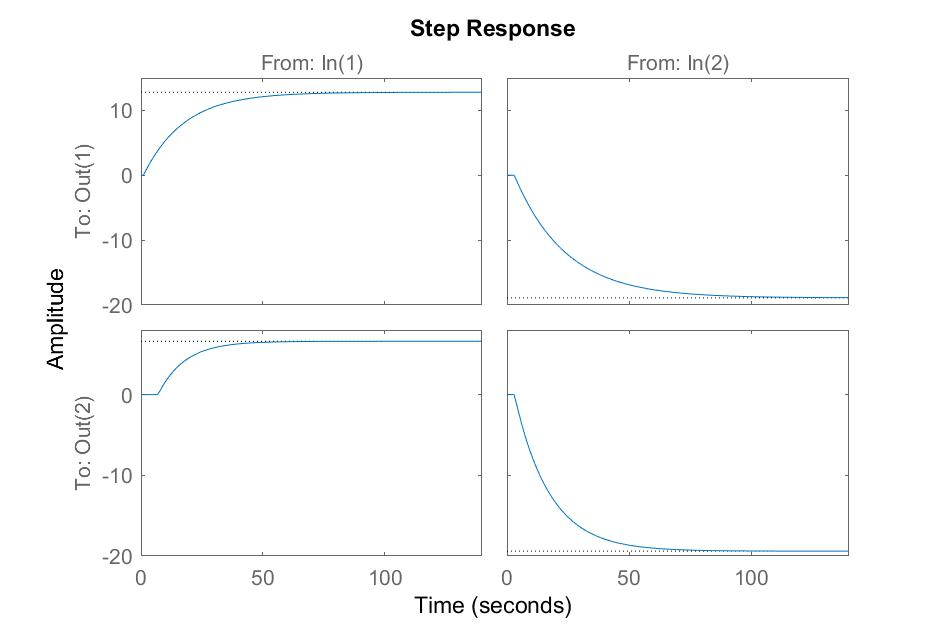
\includegraphics[width=16cm]{StepResponse.jpg}
	\centering
	\caption{Plant Step Response}
	\label{fig:StepResponse}
\end{figure}

\begin{problem}{6} Document the control horizon that you have chosen. \end{problem}

The control steps are computed with blocking, so that control steps are maintained over a few simulation samples. The control horizon is defined as
\begin{equation}
C = N_B \times N_C,
\end{equation}
where $N_B$ is the amount of samples that each control step needs to be maintained for and $C$ is the control horizon. The prediction horizon is determined from
\begin{equation}
N_P = C + \frac{L}{T_s},
\end{equation}
where $L$ is the longest plant dynamics in seconds. After the full MPC Simulink implementation was completed, these parameters where tuned to produce the desired plant response. The chosen values are $N_C=3$, $N_B=6$ and $N_P=118$ (longest plant dynamics rounded to $100 \,s$ and $T_s=1 \,s$). Maintaining each of the three inputs for six samples allows each input to be maintained almost as long as the longest plant delay (seven samples, as seen in (\ref{eq5})). %TODO what is the effect of blocking

Note that these parameters are only relevant to the prediction simulation. In each time instance of the physical system, the MPC algorithm is repeated to compute the optimal control input. The control input sent into the plant is not maintained as it is done in the prediction simulation (blocking implementation). %TODO add graph of measured and simulated signals

\section{MPC Algorithm Implementation}
\label{code:mpcimplementation}

\begin{problem}{7} Code the Matlab function \textit{ObjFunc} that calculates the objective value that will be optimized by \textit{fminunc}. Your MPC controller must implement blocking to allow for a smooth closed loop MV trajectory. \end{problem}

\begin{problem}{8} Show the code to simulate the model predictions in your objective function using the $ A, B, C $ and $ D $ matrices of the discrete time state-space model explicitly and not \textit{lsim}. \end{problem}

This section answers both \textbf{Problem 7} and \textbf{8}, as they are difficult to explain separately. 

\subsection{MPC Algorithm Description}

As mentioned in Section \ref{code:mpcDesc}, the MPC algorithm computes the optimal input steps to produce the desired future output (or manipulated variables). The MPC algorithm can be summarized in the following steps:
\begin{enumerate}
	\item Guess the optimal future inputs.
	\item Predict the future output based on the guessed inputs, from (\ref{eq6}) and (\ref{eq7}). 
	\item Compute the quadratic penalty (cost) due to the difference of the output to the setpoints and the difference between input steps, as described by the objective function defined in (\ref{eq3}).
	\item Repeat step 1 to 3 to find the optimal input steps.
\end{enumerate}

These steps are followed within MATLAB's \textit{fminunc} function. This function will numerically compute the optimal input steps to minimize the objective function.

The implementation of the MPC algorithm can be seen in Section \ref{code:mpc}. The computation of the objective function can be seen in Section \ref{code:objectiveFunc}. The implementation of the output prediction can be seen in Section \ref{code:prediction}.

\subsection{Testing the MPC Algorithm}

A script to test the MPC algorithm, for the plant in (\ref{eq1}) starting from rest with a [5,-5] setpoint, can be seen in Section \ref{code:TestMPC}. The result of this test can be seen in Figure \ref{fig:TestMPC}.

The \textit{fminunc} function computes the optimal input steps for this test script to be
\begin{align}
U^* &= \begin{bmatrix}
u^*_1(k|k) & u^*_1(k+1|k) & u^*_1(k+3|k) \\
u^*_2(k|k) & u^*_2(k+1|k) & u^*_2(k+3|k)
\end{bmatrix} \label{eq12}\\
&= \begin{bmatrix}
2.6358 & 1.7465 & 1.5409 \\
1.2987 & 1.1848 & 0.7853
\end{bmatrix}. \nonumber
\end{align}
Note that the first two input steps are maintained for six samples each, as specified by the blocking parameter $N_B=6$, and the last input step is maintained for the full duration of the prediction horizon. The plot is limited to 60 samples, but the prediction horizon is $N_P=118$, as specified.

\begin{figure}[h!]
	% This file was created by matlab2tikz.
%
%The latest updates can be retrieved from
%  http://www.mathworks.com/matlabcentral/fileexchange/22022-matlab2tikz-matlab2tikz
%where you can also make suggestions and rate matlab2tikz.
%
\definecolor{mycolor1}{rgb}{0.00000,0.44700,0.74100}%
\definecolor{mycolor2}{rgb}{0.85000,0.32500,0.09800}%
\definecolor{mycolor3}{rgb}{0.92900,0.69400,0.12500}%
\definecolor{mycolor4}{rgb}{0.49400,0.18400,0.55600}%
%
\begin{tikzpicture}

\begin{axis}[%
width=4.844in,
height=3.396in,
at={(0.813in,0.458in)},
scale only axis,
xmin=0,
xmax=60,
xlabel style={font=\color{white!15!black}},
xlabel={Samples from system discrete time k},
ymin=-6,
ymax=6,
axis background/.style={fill=white},
title style={font=\bfseries},
title={MPC Optimized Input and Predicted Output},
legend style={at={(0.97,0.5)}, anchor=east, legend cell align=left, align=left, draw=white!15!black}
]
\addplot[const plot, color=mycolor1] table[row sep=crcr] {%
0	0\\
1	0\\
2	1.48794043661385\\
3	2.88939779705764\\
4	3.26387369107736\\
5	3.60559739570094\\
6	3.91698346838632\\
7	4.20028236706281\\
8	4.4121790166945\\
9	4.60267848197739\\
10	4.67871058944432\\
11	4.74096649138508\\
12	4.79068202744093\\
13	4.82900097209096\\
14	4.56328524012395\\
15	4.30527943072257\\
16	4.40181912724793\\
17	4.48974722174962\\
18	4.5697037739367\\
19	4.64228515294933\\
20	4.70804687851057\\
21	4.76750628291091\\
22	4.82114500489206\\
23	4.86941132582231\\
24	4.91272235792336\\
25	4.95146609371335\\
26	4.98600332527193\\
27	5.01666944140799\\
28	5.0437761103169\\
29	5.06761285485067\\
30	5.0884485270882\\
31	5.10653268848393\\
32	5.122096901488\\
33	5.13535593817\\
34	5.14650891103882\\
35	5.155740330932\\
36	5.16322109654864\\
37	5.16910941991824\\
38	5.17355169183375\\
39	5.17668329102856\\
40	5.17862934064429\\
41	5.17950541531669\\
42	5.17941820200204\\
43	5.17846611747238\\
44	5.17673988522738\\
45	5.17432307439957\\
46	5.17129260307035\\
47	5.1677192082635\\
48	5.16366788474237\\
49	5.15919829460419\\
50	5.15436514954099\\
51	5.14921856751972\\
52	5.14380440552483\\
53	5.13816456990372\\
54	5.13233730575899\\
55	5.1263574667409\\
56	5.12025676650859\\
57	5.11406401304856\\
58	5.10780532696456\\
59	5.10150434478236\\
60	5.09518240824725\\
61	5.08885874053045\\
62	5.0825506102022\\
63	5.07627348377534\\
64	5.07004116757198\\
65	5.06386593961797\\
66	5.05775867222519\\
67	5.05172894587932\\
68	5.04578515501148\\
69	5.03993460619517\\
70	5.03418360927499\\
71	5.02853756190133\\
72	5.02300102791454\\
73	5.01757780999375\\
74	5.01227101695835\\
75	5.0070831260854\\
76	5.00201604078242\\
77	4.99707114393312\\
78	4.99224934721287\\
79	4.9875511366515\\
80	4.98297661470254\\
81	4.97852553906155\\
82	4.97419735845973\\
83	4.96999124564446\\
84	4.96590612774428\\
85	4.96194071420297\\
86	4.9580935224548\\
87	4.95436290150182\\
88	4.9507470535435\\
89	4.94724405379845\\
90	4.94385186864911\\
91	4.94056837223132\\
92	4.93739136158226\\
93	4.93431857045297\\
94	4.93134768188398\\
95	4.92847633963642\\
96	4.92570215856404\\
97	4.92302273400638\\
98	4.92043565027715\\
99	4.91793848831737\\
100	4.91552883257756\\
101	4.91320427718895\\
102	4.91096243147961\\
103	4.90880092488721\\
104	4.90671741131678\\
105	4.90470957298812\\
106	4.90277512381456\\
107	4.9009118123517\\
108	4.89911742435196\\
109	4.89738978495819\\
110	4.89572676056733\\
111	4.89412626039248\\
112	4.89258623775015\\
113	4.89110469109706\\
114	4.88967966483921\\
115	4.88830924993441\\
116	4.88699158430742\\
117	4.88572485309599\\
118	4.88450728874408\\
};
\addlegendentry{$y_1^*(k|k)$}

\addplot[const plot, color=mycolor2] table[row sep=crcr] {%
0	0\\
1	0\\
2	0\\
3	0\\
4	-1.4001567514518\\
5	-2.70637973129799\\
6	-3.92497077212905\\
7	-5.06180892894096\\
8	-4.96526000697591\\
9	-4.89899316528328\\
10	-4.99917770497963\\
11	-5.11245530488457\\
12	-5.23621065031048\\
13	-5.36815614282112\\
14	-5.54161193833568\\
15	-5.71643227743428\\
16	-5.37765223875477\\
17	-5.07242213809773\\
18	-4.79754252696954\\
19	-4.55011176065993\\
20	-4.55589582469796\\
21	-4.56409084085963\\
22	-4.57428970186057\\
23	-4.58613412093886\\
24	-4.59930947113619\\
25	-4.61354013608082\\
26	-4.62858532346792\\
27	-4.64423529697777\\
28	-4.66030798649968\\
29	-4.67664594027957\\
30	-4.69311358601403\\
31	-4.70959477100633\\
32	-4.72599055430724\\
33	-4.74221722631272\\
34	-4.75820453360421\\
35	-4.77389408891719\\
36	-4.78923794802937\\
37	-4.80419733708885\\
38	-4.8187415154712\\
39	-4.83284676067697\\
40	-4.84649546307182\\
41	-4.85967531944078\\
42	-4.87237861538926\\
43	-4.88460158758463\\
44	-4.89634385770318\\
45	-4.90760793073695\\
46	-4.91839875102966\\
47	-4.92872331005882\\
48	-4.93859030056711\\
49	-4.94800981217742\\
50	-4.95699306410584\\
51	-4.96555217102197\\
52	-4.97369993849887\\
53	-4.9814496848507\\
54	-4.98881508647759\\
55	-4.99581004412766\\
56	-5.00244856774902\\
57	-5.00874467784127\\
58	-5.01471232143058\\
59	-5.02036530098542\\
60	-5.02571721476457\\
61	-5.03078140724636\\
62	-5.03557092842984\\
63	-5.0400985009265\\
64	-5.04437649387635\\
65	-5.04841690282582\\
66	-5.05223133479821\\
67	-5.05583099787164\\
68	-5.05922669465467\\
69	-5.06242881911768\\
70	-5.06544735629926\\
71	-5.06829188446111\\
72	-5.07097157931449\\
73	-5.07349521998479\\
74	-5.07587119642053\\
75	-5.07810751798812\\
76	-5.08021182302537\\
77	-5.08219138915472\\
78	-5.08405314418259\\
79	-5.08580367743344\\
80	-5.08744925138707\\
81	-5.08899581350577\\
82	-5.09044900815333\\
83	-5.09181418852226\\
84	-5.09309642849774\\
85	-5.09430053439809\\
86	-5.09543105654095\\
87	-5.09649230059321\\
88	-5.09748833867004\\
89	-5.09842302015521\\
90	-5.09929998222045\\
91	-5.10012266002679\\
92	-5.10089429659539\\
93	-5.10161795233878\\
94	-5.10229651424715\\
95	-5.10293270472705\\
96	-5.10352909009213\\
97	-5.1040880887079\\
98	-5.10461197879407\\
99	-5.10510290588959\\
100	-5.10556288998662\\
101	-5.10599383234089\\
102	-5.10639752196648\\
103	-5.10677564182378\\
104	-5.10712977471006\\
105	-5.10746140886206\\
106	-5.10777194328077\\
107	-5.10806269278823\\
108	-5.10833489282658\\
109	-5.10858970400963\\
110	-5.10882821643675\\
111	-5.10905145377941\\
112	-5.10926037714993\\
113	-5.1094558887622\\
114	-5.10963883539393\\
115	-5.10981001165935\\
116	-5.10997016310159\\
117	-5.11011998911326\\
118	-5.11026014569366\\
};
\addlegendentry{$y_2^*(k|k)$}

\addplot[const plot, color=mycolor3] table[row sep=crcr] {%
0	0.999999993637481\\
1	0.999999993637481\\
2	0.999999993637481\\
3	0.999999993637481\\
4	0.999999993637481\\
5	0.999999993637481\\
6	0.938959813609464\\
7	0.938959813609464\\
8	0.938959813609464\\
9	0.938959813609464\\
10	0.938959813609464\\
11	0.938959813609464\\
12	0.54419120806217\\
13	0.54419120806217\\
14	0.54419120806217\\
15	0.54419120806217\\
16	0.54419120806217\\
17	0.54419120806217\\
18	0.54419120806217\\
19	0.54419120806217\\
20	0.54419120806217\\
21	0.54419120806217\\
22	0.54419120806217\\
23	0.54419120806217\\
24	0.54419120806217\\
25	0.54419120806217\\
26	0.54419120806217\\
27	0.54419120806217\\
28	0.54419120806217\\
29	0.54419120806217\\
30	0.54419120806217\\
31	0.54419120806217\\
32	0.54419120806217\\
33	0.54419120806217\\
34	0.54419120806217\\
35	0.54419120806217\\
36	0.54419120806217\\
37	0.54419120806217\\
38	0.54419120806217\\
39	0.54419120806217\\
40	0.54419120806217\\
41	0.54419120806217\\
42	0.54419120806217\\
43	0.54419120806217\\
44	0.54419120806217\\
45	0.54419120806217\\
46	0.54419120806217\\
47	0.54419120806217\\
48	0.54419120806217\\
49	0.54419120806217\\
50	0.54419120806217\\
51	0.54419120806217\\
52	0.54419120806217\\
53	0.54419120806217\\
54	0.54419120806217\\
55	0.54419120806217\\
56	0.54419120806217\\
57	0.54419120806217\\
58	0.54419120806217\\
59	0.54419120806217\\
60	0.54419120806217\\
61	0.54419120806217\\
62	0.54419120806217\\
63	0.54419120806217\\
64	0.54419120806217\\
65	0.54419120806217\\
66	0.54419120806217\\
67	0.54419120806217\\
68	0.54419120806217\\
69	0.54419120806217\\
70	0.54419120806217\\
71	0.54419120806217\\
72	0.54419120806217\\
73	0.54419120806217\\
74	0.54419120806217\\
75	0.54419120806217\\
76	0.54419120806217\\
77	0.54419120806217\\
78	0.54419120806217\\
79	0.54419120806217\\
80	0.54419120806217\\
81	0.54419120806217\\
82	0.54419120806217\\
83	0.54419120806217\\
84	0.54419120806217\\
85	0.54419120806217\\
86	0.54419120806217\\
87	0.54419120806217\\
88	0.54419120806217\\
89	0.54419120806217\\
90	0.54419120806217\\
91	0.54419120806217\\
92	0.54419120806217\\
93	0.54419120806217\\
94	0.54419120806217\\
95	0.54419120806217\\
96	0.54419120806217\\
97	0.54419120806217\\
98	0.54419120806217\\
99	0.54419120806217\\
100	0.54419120806217\\
101	0.54419120806217\\
102	0.54419120806217\\
103	0.54419120806217\\
104	0.54419120806217\\
105	0.54419120806217\\
106	0.54419120806217\\
107	0.54419120806217\\
108	0.54419120806217\\
109	0.54419120806217\\
110	0.54419120806217\\
111	0.54419120806217\\
112	0.54419120806217\\
113	0.54419120806217\\
114	0.54419120806217\\
115	0.54419120806217\\
116	0.54419120806217\\
117	0.54419120806217\\
118	0.54419120806217\\
};
\addlegendentry{$u_1^*(k|k)$}

\addplot[const plot, color=mycolor4] table[row sep=crcr] {%
0	2.07579575795987\\
1	2.07579575795987\\
2	2.07579575795987\\
3	2.07579575795987\\
4	2.07579575795987\\
5	2.07579575795987\\
6	2.18358427038044\\
7	2.18358427038044\\
8	2.18358427038044\\
9	2.18358427038044\\
10	2.18358427038044\\
11	2.18358427038044\\
12	1.78886239090085\\
13	1.78886239090085\\
14	1.78886239090085\\
15	1.78886239090085\\
16	1.78886239090085\\
17	1.78886239090085\\
18	1.78886239090085\\
19	1.78886239090085\\
20	1.78886239090085\\
21	1.78886239090085\\
22	1.78886239090085\\
23	1.78886239090085\\
24	1.78886239090085\\
25	1.78886239090085\\
26	1.78886239090085\\
27	1.78886239090085\\
28	1.78886239090085\\
29	1.78886239090085\\
30	1.78886239090085\\
31	1.78886239090085\\
32	1.78886239090085\\
33	1.78886239090085\\
34	1.78886239090085\\
35	1.78886239090085\\
36	1.78886239090085\\
37	1.78886239090085\\
38	1.78886239090085\\
39	1.78886239090085\\
40	1.78886239090085\\
41	1.78886239090085\\
42	1.78886239090085\\
43	1.78886239090085\\
44	1.78886239090085\\
45	1.78886239090085\\
46	1.78886239090085\\
47	1.78886239090085\\
48	1.78886239090085\\
49	1.78886239090085\\
50	1.78886239090085\\
51	1.78886239090085\\
52	1.78886239090085\\
53	1.78886239090085\\
54	1.78886239090085\\
55	1.78886239090085\\
56	1.78886239090085\\
57	1.78886239090085\\
58	1.78886239090085\\
59	1.78886239090085\\
60	1.78886239090085\\
61	1.78886239090085\\
62	1.78886239090085\\
63	1.78886239090085\\
64	1.78886239090085\\
65	1.78886239090085\\
66	1.78886239090085\\
67	1.78886239090085\\
68	1.78886239090085\\
69	1.78886239090085\\
70	1.78886239090085\\
71	1.78886239090085\\
72	1.78886239090085\\
73	1.78886239090085\\
74	1.78886239090085\\
75	1.78886239090085\\
76	1.78886239090085\\
77	1.78886239090085\\
78	1.78886239090085\\
79	1.78886239090085\\
80	1.78886239090085\\
81	1.78886239090085\\
82	1.78886239090085\\
83	1.78886239090085\\
84	1.78886239090085\\
85	1.78886239090085\\
86	1.78886239090085\\
87	1.78886239090085\\
88	1.78886239090085\\
89	1.78886239090085\\
90	1.78886239090085\\
91	1.78886239090085\\
92	1.78886239090085\\
93	1.78886239090085\\
94	1.78886239090085\\
95	1.78886239090085\\
96	1.78886239090085\\
97	1.78886239090085\\
98	1.78886239090085\\
99	1.78886239090085\\
100	1.78886239090085\\
101	1.78886239090085\\
102	1.78886239090085\\
103	1.78886239090085\\
104	1.78886239090085\\
105	1.78886239090085\\
106	1.78886239090085\\
107	1.78886239090085\\
108	1.78886239090085\\
109	1.78886239090085\\
110	1.78886239090085\\
111	1.78886239090085\\
112	1.78886239090085\\
113	1.78886239090085\\
114	1.78886239090085\\
115	1.78886239090085\\
116	1.78886239090085\\
117	1.78886239090085\\
118	1.78886239090085\\
};
\addlegendentry{$u_2^*(k|k)$}

\end{axis}
\end{tikzpicture}%
	%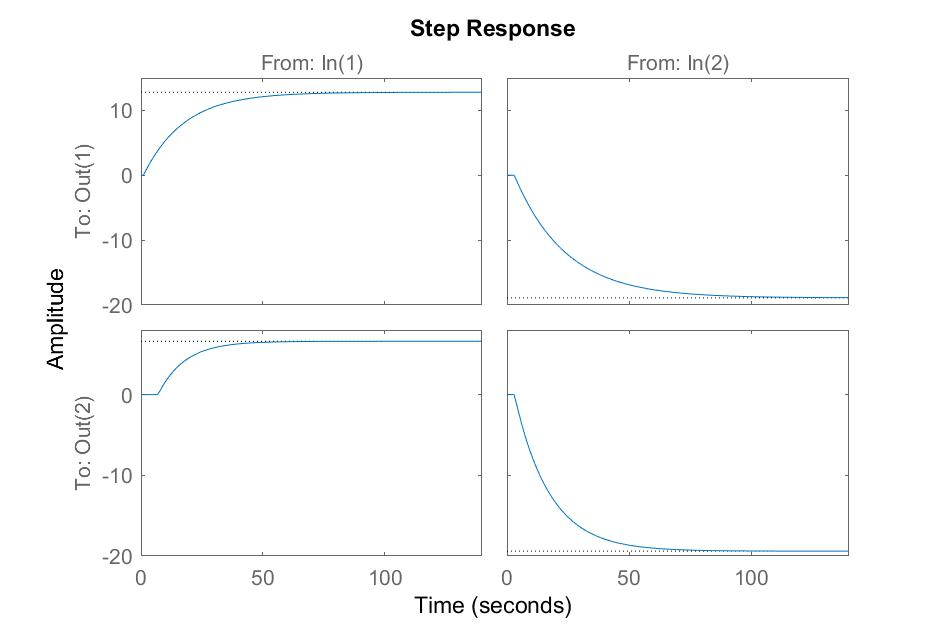
\includegraphics[width=17.5cm]{StepResponse.jpg}
	\centering
	\caption{MPC Test Result}
	\label{fig:TestMPC}
\end{figure}

\subsection{Delayed Input Implementation}

From the prediction algorithm in (\ref{eq6}) and (\ref{eq9a}) it is seen that the past input steps are needed. A circular buffer is used to store the past implemented inputs, as follows:
\begin{equation}
U_{stored} = \begin{bmatrix}
u^*_1(k|k) & u^*_1(k-1|k) & u^*_1(k-2|k) & u^*_1(k-3|k) \\
u^*_2(k|k) & u^*_2(k-1|k) & u^*_2(k-2|k) & u^*_2(k-3|k) \\
\end{bmatrix}, \label{eq13}
\end{equation}
from which $u_{delayed}(k)$, as seen in (\ref{eq9a}), can be determined from:
\begin{equation}
u_{delayed}(k) =
\begin{bmatrix}
U_{stored}(row \, 1, column \, 2) \\
U_{stored}(row \, 2, column \, 4)
\end{bmatrix}. \label{eq14}
\end{equation}
Before the next iteration of the prediction algorithm, the buffer is shifted by one sample (or one column to the right). At the start of the next iteration, the first column of the buffer is filled with the input step of that iteration. A buffer created and shifted similarly for the $z(k)$ parameter in (\ref{eq6}). These implementations can be seen in Section \ref{code:prediction}.

\section{Simulink Model Implementation}

\begin{problem}{9} Code a MATLAB Simulink s-function m-file to call \textit{fminunc} on your function ObjFunc and connect it to the original continuous-time model G(s). \end{problem}

\subsection{Simulink Model Description}

A Simulink model was created to model MPC control of the plant, as can be seen in Figure \ref{fig:FullModel}. The continuous plant block is an implementation of (\ref{eq1}), as can be seen in Figure \ref{fig:ContinuousPlant}. The MPC algorithm reads the states of the plant at each step. The states are determined from the discrete plant block, which is a discrete state space implementation of the plant, as seen in Figure \ref{fig:DiscretePlant}. The MPC algorithm is implemented within the MPC block.

The sampling time for the discrete plant and for the MPC block is 1 second. The Simulink \textit{solver options} are therefore set to use \textit{Runge-Kutta} with a \textit{fixed-step size} of 1 second.

\begin{figure}[h!]
	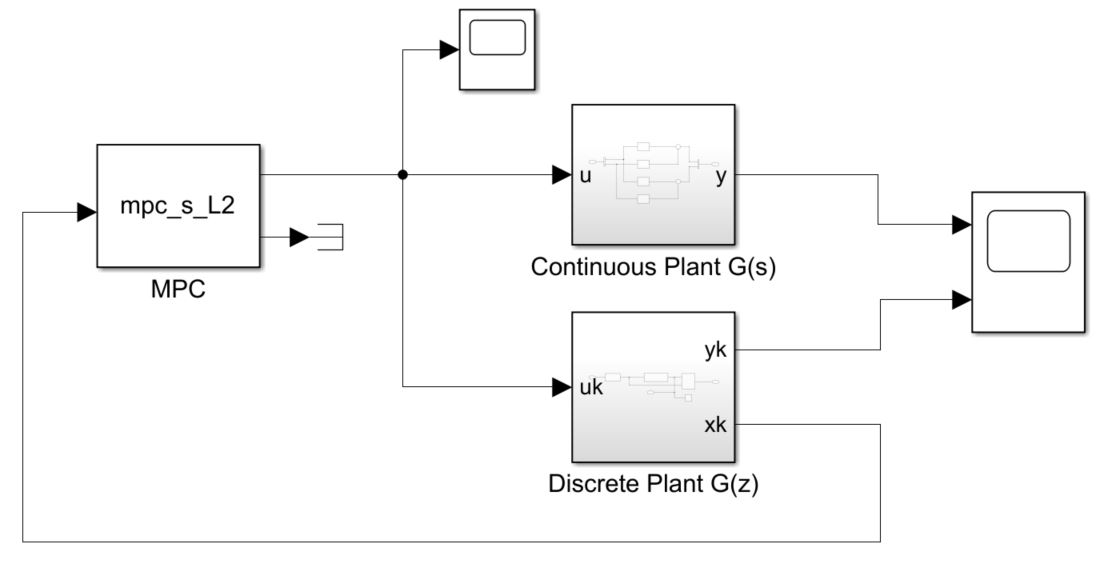
\includegraphics[width=14cm]{FullModel.jpg}
	\centering
	\caption{Full Simulink Model}
	\label{fig:FullModel}
\end{figure}

\begin{figure}[h!]
	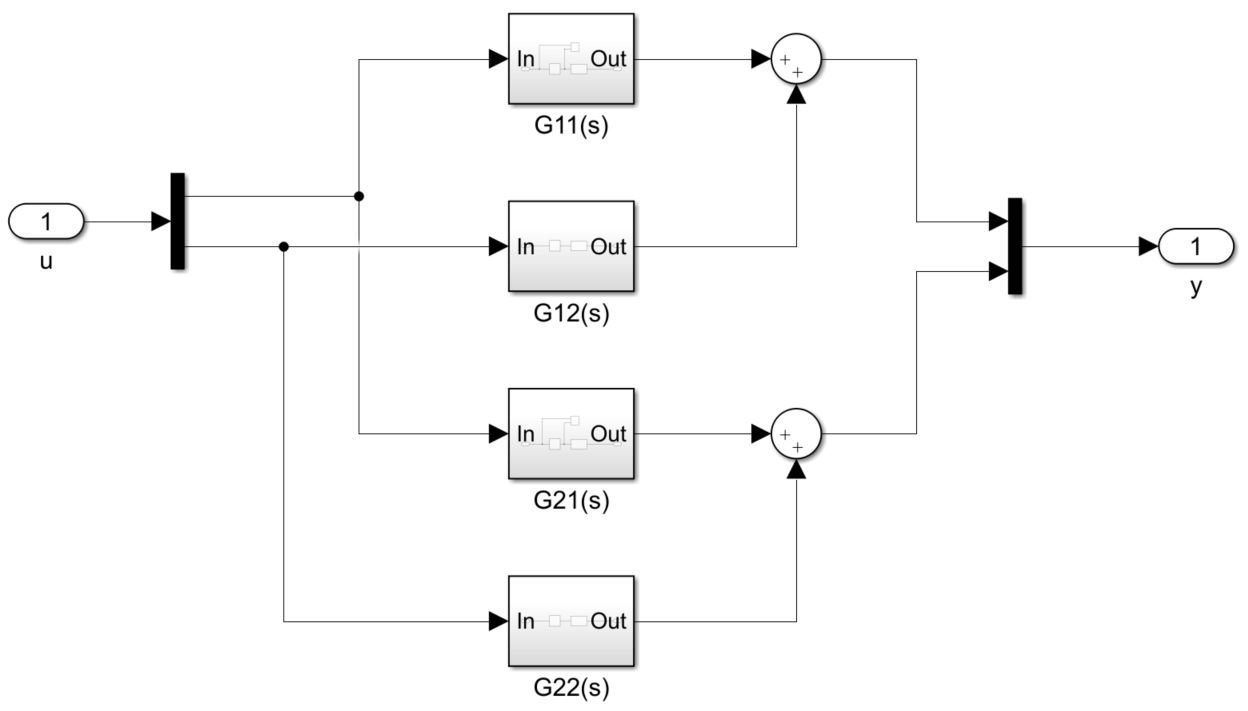
\includegraphics[width=15cm]{ContinuousPlant.jpg}
	\centering
	\caption{Simulink Continuous Plant Block}
	\label{fig:ContinuousPlant}
\end{figure}

\subsection{MPC Block Coding}

The MPC algorithm is run in the Simulink model by using a level-2 MATLAB s-function block, as seen in Figure \ref{fig:FullModel}. This block allows the use of MATLAB language to create a custom block. A template for creating a m-file to define the workings of the block can be invoked by typing \textit{edit msfuntmpl\_basic} in the \textit{Command Window}. The definition of the MPC block can be seen in Section \ref{code:mpcL2}.

\subsubsection{Block Setup}

At the start of the Simulation, the \textit{SetupParameters} function (Section \ref{code:Setup}) is called to create and define the discrete model in (\ref{eq5}), the setpoint vector array, the control \& prediction horizon, weighing matrices and the sample time. This is done by setting the Simulink \textit{InitFcn} callback to the \textit{SetupParameters} function. These parameters are passed to the MPC block as dialog parameters.

The basic characteristics of the MPC block, such as the amount of inputs and outputs, are defined in the \textit{setup} function, as seen in Section \ref{code:mpcL2}. Storage of data within the block is done in the block's \textit{Dwork} vectors. The size and amount of \textit{Dwork} vectors have to be defined in the \textit{DoPostPropSetup} function.

At the start of the Simulink simulation, the MPC block's \textit{start} function is called. In this function, the state space parameters in (\ref{eq8}) and (\ref{eq9}) are determined, flattened and stored in the \textit{Dwork} vectors.

At the start of the prediction simulation, the values for previously implemented parameters $u(k)$ and $z(k)$ are needed, as can be seen from (\ref{eq6d}) and (\ref{eq9a}). The required storage sizes are set in the \textit{DoPostPropSetup} function and the vectors are initialized to zero at the start of the simulation in the \textit{start} function.
	
\subsubsection{Code Execution During Simulation}

During each Simulink simulation step, the \textit{Outputs} function is called in the MPC block, as seen in Section \ref{code:mpcL2}. This function reads the current state from the Simulink environment and determines the output setpoint based on the current simulation time. These parameters, as well as the plant model parameters, system parameters and stored parameters are passed to the \textit{mpc} function. The \textit{mpc} function, as seen in Section \ref{code:mpc}, then calculates the optimal control steps to deliver the desired future response, as was described in Section \ref{code:mpcimplementation}.

The difference between the MPC implementation during simulation and for the test function (as in Section \ref{code:TestMPC}, result in Figure \ref{fig:TestMPC}), is that the current states and previously implemented parameters $u(k)$ and $z(k)$, as can be seen from (\ref{eq6d}) and (\ref{eq9a}), are not zero. For the full simulation, the output setpoint changes from [5,-5] to [-5,5] at simulation discrete time of 100 (step 101), as described in \textbf{Problem 10}. The optimal future input and output calculated by the MPC algorithm at this step can be seen in Figure \ref{fig:MPCduringSim}. 

At the start of the prediction algorithm for the Simulink time of 100 (step 101), the input buffer in (\ref{eq13}) must have the previously implemented simulation step inputs stored, as follows:
\begin{equation}
U_{stored} = \begin{bmatrix}
u^*_1(100|100) & u^*_1(99|100) & u^*_1(98|100) & u^*_1(97|100) \\
u^*_1(100|100) & u^*_1(99|100) & u^*_1(98|100) & u^*_1(97|100) \\
\end{bmatrix}. \label{eq15}
\end{equation}
This is done by saving the current input (to be implemented for the current Simulink step) in the first column of the buffer after the MPC calculation is complete. At the start of the next Simulink step, the buffer is shifted one column to the right. Similar logic is followed with the storage of $z(k)$. This implementation can be seen in Section \ref{code:mpcL2}.

\begin{figure}[h!]
	% This file was created by matlab2tikz.
%
%The latest updates can be retrieved from
%  http://www.mathworks.com/matlabcentral/fileexchange/22022-matlab2tikz-matlab2tikz
%where you can also make suggestions and rate matlab2tikz.
%
\definecolor{mycolor1}{rgb}{0.00000,0.44700,0.74100}%
\definecolor{mycolor2}{rgb}{0.85000,0.32500,0.09800}%
\definecolor{mycolor3}{rgb}{0.92900,0.69400,0.12500}%
\definecolor{mycolor4}{rgb}{0.49400,0.18400,0.55600}%
%
\begin{tikzpicture}

\begin{axis}[%
width=4.844in,
height=3.396in,
at={(0.812in,0.458in)},
scale only axis,
xmin=0,
xmax=100,
xlabel style={font=\color{white!15!black}},
xlabel={Samples from Simulink discrete time 150},
ymin=-6,
ymax=6,
axis background/.style={fill=white},
title style={font=\bfseries},
title={MPC Optimized Input and Predicted Output for Simulink Time at 150},
legend style={at={(0.97,0.5)}, anchor=east, legend cell align=left, align=left, draw=white!15!black}
]
\addplot[const plot, color=mycolor1] table[row sep=crcr] {%
0	-0.281927243096071\\
1	-0.408479416595808\\
2	1.14787323280938\\
3	2.74080372899207\\
4	3.31416323248213\\
5	3.84353790098771\\
6	4.33197995679286\\
7	4.78234116702012\\
8	4.91599197524328\\
9	5.03306374475392\\
10	5.01279315514139\\
11	4.98427108040546\\
12	4.94841562710495\\
13	4.90607114702511\\
14	4.6131474193863\\
15	4.32945496593508\\
16	4.42012627410682\\
17	4.50268607023109\\
18	4.57773795330099\\
19	4.64584429478549\\
20	4.70752892063235\\
21	4.76327962409766\\
22	4.81355051985268\\
23	4.85876424918277\\
24	4.89931404549488\\
25	4.93556566878883\\
26	4.96785921721893\\
27	4.99651082337725\\
28	5.02181424246278\\
29	5.04404233906339\\
30	5.06344847886563\\
31	5.0802678312207\\
32	5.09471858813166\\
33	5.10700310488594\\
34	5.11730896723594\\
35	5.12580998972993\\
36	5.13266714951217\\
37	5.13802945964543\\
38	5.14203478575951\\
39	5.14481060959476\\
40	5.14647474278962\\
41	5.14713599405389\\
42	5.14689479267578\\
43	5.14584377112786\\
44	5.14406830936608\\
45	5.14164704325493\\
46	5.138652339401\\
47	5.13515073853515\\
48	5.13120336945062\\
49	5.12686633537917\\
50	5.12219107457021\\
51	5.11722469672758\\
52	5.11201029685518\\
53	5.10658724796597\\
54	5.10099147401726\\
55	5.09525570435001\\
56	5.0894097108297\\
57	5.0834805288108\\
58	5.0774926629764\\
59	5.07146827903813\\
60	5.0654273822195\\
61	5.05938798338725\\
62	5.05336625364058\\
63	5.04737666811694\\
64	5.0414321397247\\
65	5.03554414346786\\
66	5.02972283198582\\
67	5.02397714289114\\
68	5.01831489845119\\
69	5.01274289812469\\
70	5.00726700443107\\
71	5.00189222260035\\
72	4.99662277442193\\
73	4.9914621666841\\
74	4.98641325457054\\
75	4.9814783003565\\
76	4.97665902772503\\
77	4.97195667200294\\
78	4.96737202659649\\
79	4.9629054858887\\
80	4.95855708484298\\
81	4.95432653554169\\
82	4.95021326087329\\
83	4.94621642556768\\
84	4.94233496476606\\
85	4.9385676102995\\
86	4.93491291483854\\
87	4.93136927406573\\
88	4.92793494701258\\
89	4.92460807469302\\
90	4.92138669715673\\
91	4.91826876907722\\
92	4.91525217398186\\
93	4.9123347372239\\
94	4.90951423778952\\
95	4.90678841902687\\
96	4.90415499837784\\
97	4.90161167618797\\
98	4.89915614366469\\
99	4.89678609004904\\
100	4.89449920906185\\
};
\addlegendentry{$y_1^*(k|k)$}

\addplot[const plot, color=mycolor2] table[row sep=crcr] {%
0	-0.265427567383959\\
1	-0.436160817055089\\
2	-0.604232664244252\\
3	-0.588848010715861\\
4	-1.96203113953449\\
5	-3.26011657766015\\
6	-4.46981294678161\\
7	-5.55301448085787\\
8	-5.26397370404803\\
9	-5.02125694984734\\
10	-5.0002584776284\\
11	-5.00308666307356\\
12	-5.02617785670745\\
13	-5.06637975475729\\
14	-5.33966081360182\\
15	-5.60563948148944\\
16	-5.32288364978686\\
17	-5.06827956822009\\
18	-4.83913367327532\\
19	-4.63300366684455\\
20	-4.63809917314209\\
21	-4.64529704714322\\
22	-4.65424198394653\\
23	-4.6646212976054\\
24	-4.67616041544454\\
25	-4.68861881898354\\
26	-4.7017863888537\\
27	-4.7154801150618\\
28	-4.72954113755959\\
29	-4.7438320853513\\
30	-4.75823468534533\\
31	-4.77264761485612\\
32	-4.78698457411406\\
33	-4.80117255736683\\
34	-4.81515030317593\\
35	-4.82886690634588\\
36	-4.84228057558735\\
37	-4.85535752252542\\
38	-4.86807096903347\\
39	-4.88040026111592\\
40	-4.89233007868918\\
41	-4.90384973163202\\
42	-4.9149525334026\\
43	-4.92563524435862\\
44	-4.93589757767795\\
45	-4.94574176146622\\
46	-4.95517215126216\\
47	-4.964194887717\\
48	-4.97281759473605\\
49	-4.98104911383426\\
50	-4.98889927087697\\
51	-4.99637867175633\\
52	-5.00349852389768\\
53	-5.01027048080017\\
54	-5.01670650709695\\
55	-5.02281876187372\\
56	-5.02861949821377\\
57	-5.03412097714479\\
58	-5.03933539434942\\
59	-5.04427481817052\\
60	-5.04895113759437\\
61	-5.05337601903226\\
62	-5.05756087084482\\
63	-5.06151681466515\\
64	-5.06525466267728\\
65	-5.06878490009688\\
66	-5.07211767218306\\
67	-5.07526277518285\\
68	-5.07822965067634\\
69	-5.08102738284942\\
70	-5.08366469827433\\
71	-5.08614996782605\\
72	-5.08849121040517\\
73	-5.09069609817655\\
74	-5.09277196306725\\
75	-5.09472580429803\\
76	-5.09656429675032\\
77	-5.09829379999507\\
78	-5.09992036783172\\
79	-5.10144975820553\\
80	-5.10288744338831\\
81	-5.10423862032366\\
82	-5.10550822105135\\
83	-5.10670092313772\\
84	-5.10782116004987\\
85	-5.10887313142105\\
86	-5.10986081316302\\
87	-5.11078796738865\\
88	-5.11165815211483\\
89	-5.11247473072111\\
90	-5.11324088114494\\
91	-5.11395960479865\\
92	-5.11463373519708\\
93	-5.11526594628828\\
94	-5.11585876048236\\
95	-5.11641455637641\\
96	-5.1169355761751\\
97	-5.11742393280878\\
98	-5.11788161675211\\
99	-5.11831050254785\\
100	-5.11871235504119\\
};
\addlegendentry{$y_2^*(k|k)$}

\addplot[const plot, color=mycolor3] table[row sep=crcr] {%
0	0.999999990419406\\
1	0.999999990419406\\
2	0.999999990419406\\
3	0.999999990419406\\
4	0.999999990419406\\
5	0.999999990419406\\
6	0.621902072597912\\
7	0.621902072597912\\
8	0.621902072597912\\
9	0.621902072597912\\
10	0.621902072597912\\
11	0.621902072597912\\
12	0.292767859829708\\
13	0.292767859829708\\
14	0.292767859829708\\
15	0.292767859829708\\
16	0.292767859829708\\
17	0.292767859829708\\
18	0.292767859829708\\
19	0.292767859829708\\
20	0.292767859829708\\
21	0.292767859829708\\
22	0.292767859829708\\
23	0.292767859829708\\
24	0.292767859829708\\
25	0.292767859829708\\
26	0.292767859829708\\
27	0.292767859829708\\
28	0.292767859829708\\
29	0.292767859829708\\
30	0.292767859829708\\
31	0.292767859829708\\
32	0.292767859829708\\
33	0.292767859829708\\
34	0.292767859829708\\
35	0.292767859829708\\
36	0.292767859829708\\
37	0.292767859829708\\
38	0.292767859829708\\
39	0.292767859829708\\
40	0.292767859829708\\
41	0.292767859829708\\
42	0.292767859829708\\
43	0.292767859829708\\
44	0.292767859829708\\
45	0.292767859829708\\
46	0.292767859829708\\
47	0.292767859829708\\
48	0.292767859829708\\
49	0.292767859829708\\
50	0.292767859829708\\
51	0.292767859829708\\
52	0.292767859829708\\
53	0.292767859829708\\
54	0.292767859829708\\
55	0.292767859829708\\
56	0.292767859829708\\
57	0.292767859829708\\
58	0.292767859829708\\
59	0.292767859829708\\
60	0.292767859829708\\
61	0.292767859829708\\
62	0.292767859829708\\
63	0.292767859829708\\
64	0.292767859829708\\
65	0.292767859829708\\
66	0.292767859829708\\
67	0.292767859829708\\
68	0.292767859829708\\
69	0.292767859829708\\
70	0.292767859829708\\
71	0.292767859829708\\
72	0.292767859829708\\
73	0.292767859829708\\
74	0.292767859829708\\
75	0.292767859829708\\
76	0.292767859829708\\
77	0.292767859829708\\
78	0.292767859829708\\
79	0.292767859829708\\
80	0.292767859829708\\
81	0.292767859829708\\
82	0.292767859829708\\
83	0.292767859829708\\
84	0.292767859829708\\
85	0.292767859829708\\
86	0.292767859829708\\
87	0.292767859829708\\
88	0.292767859829708\\
89	0.292767859829708\\
90	0.292767859829708\\
91	0.292767859829708\\
92	0.292767859829708\\
93	0.292767859829708\\
94	0.292767859829708\\
95	0.292767859829708\\
96	0.292767859829708\\
97	0.292767859829708\\
98	0.292767859829708\\
99	0.292767859829708\\
100	0.292767859829708\\
};
\addlegendentry{$u_1^*(k|k)$}

\addplot[const plot, color=mycolor4] table[row sep=crcr] {%
0	1.89812937938931\\
1	1.89812937938931\\
2	1.89812937938931\\
3	1.89812937938931\\
4	1.89812937938931\\
5	1.89812937938931\\
6	2.03709356449849\\
7	2.03709356449849\\
8	2.03709356449849\\
9	2.03709356449849\\
10	2.03709356449849\\
11	2.03709356449849\\
12	1.62145647440115\\
13	1.62145647440115\\
14	1.62145647440115\\
15	1.62145647440115\\
16	1.62145647440115\\
17	1.62145647440115\\
18	1.62145647440115\\
19	1.62145647440115\\
20	1.62145647440115\\
21	1.62145647440115\\
22	1.62145647440115\\
23	1.62145647440115\\
24	1.62145647440115\\
25	1.62145647440115\\
26	1.62145647440115\\
27	1.62145647440115\\
28	1.62145647440115\\
29	1.62145647440115\\
30	1.62145647440115\\
31	1.62145647440115\\
32	1.62145647440115\\
33	1.62145647440115\\
34	1.62145647440115\\
35	1.62145647440115\\
36	1.62145647440115\\
37	1.62145647440115\\
38	1.62145647440115\\
39	1.62145647440115\\
40	1.62145647440115\\
41	1.62145647440115\\
42	1.62145647440115\\
43	1.62145647440115\\
44	1.62145647440115\\
45	1.62145647440115\\
46	1.62145647440115\\
47	1.62145647440115\\
48	1.62145647440115\\
49	1.62145647440115\\
50	1.62145647440115\\
51	1.62145647440115\\
52	1.62145647440115\\
53	1.62145647440115\\
54	1.62145647440115\\
55	1.62145647440115\\
56	1.62145647440115\\
57	1.62145647440115\\
58	1.62145647440115\\
59	1.62145647440115\\
60	1.62145647440115\\
61	1.62145647440115\\
62	1.62145647440115\\
63	1.62145647440115\\
64	1.62145647440115\\
65	1.62145647440115\\
66	1.62145647440115\\
67	1.62145647440115\\
68	1.62145647440115\\
69	1.62145647440115\\
70	1.62145647440115\\
71	1.62145647440115\\
72	1.62145647440115\\
73	1.62145647440115\\
74	1.62145647440115\\
75	1.62145647440115\\
76	1.62145647440115\\
77	1.62145647440115\\
78	1.62145647440115\\
79	1.62145647440115\\
80	1.62145647440115\\
81	1.62145647440115\\
82	1.62145647440115\\
83	1.62145647440115\\
84	1.62145647440115\\
85	1.62145647440115\\
86	1.62145647440115\\
87	1.62145647440115\\
88	1.62145647440115\\
89	1.62145647440115\\
90	1.62145647440115\\
91	1.62145647440115\\
92	1.62145647440115\\
93	1.62145647440115\\
94	1.62145647440115\\
95	1.62145647440115\\
96	1.62145647440115\\
97	1.62145647440115\\
98	1.62145647440115\\
99	1.62145647440115\\
100	1.62145647440115\\
};
\addlegendentry{$u_2^*(k|k)$}

\end{axis}
\end{tikzpicture}%
	%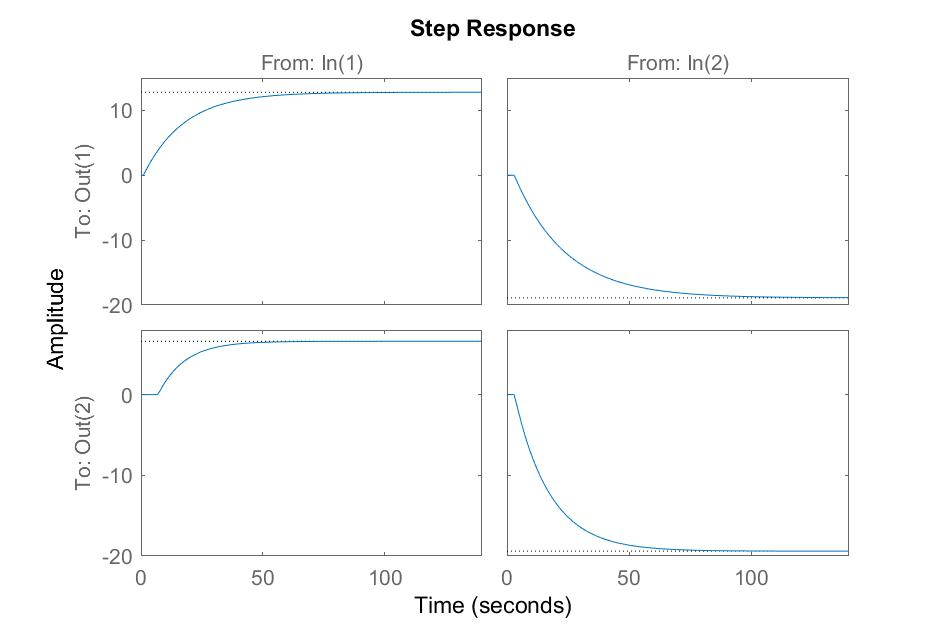
\includegraphics[width=17.5cm]{StepResponse.jpg}
	\centering
	\caption{MPC Prediction During Simulation at Simulation Step 101}
	\label{fig:MPCduringSim}
\end{figure}

To increase the speed with which \textit{fminunc} finds the optimal input steps, as described by (\ref{eq12}), the optimal input steps found by the previous Simulink simulation step is used as a first guess for the optimal inputs of the current simulation step, as seen in Section \ref{code:mpcL2} and \ref{code:mpc}.

At the end of the \textit{Outputs} function, the block output is set to the plant input to implement in the current Simulink step.

\subsection{Testing the Plant Model Implementations}

The implementation of the model of the physical system needs to be very accurate for MPC to be effective. A mistake in the model used in the prediction algorithm, as seen in Section \ref{code:prediction}, would be costly. The output of the discrete plant block is compared to the continuous plant block to verify that (\ref{eq6}) to (\ref{eq9}) produces the desired response, as seen in Figure \ref{fig:FullModel}. Both the continuous and discrete plant outputs are plotted on the simulation result plot in Figure \ref{fig:Outputs} in Section \ref{sec:Results}.

To test the implementation of (\ref{eq6}) to (\ref{eq9}) within the MPC block, the second output of the block was set to $y(k|k)$, as seen in Section \ref{code:mpcL2}. It was found that this output produced the exact same result as the discrete plant block output, confirming that the MPC implementation of the plant, as well as storages of past variables, was implemented correctly. The second output was not used thereafter, as seen in Figure \ref{fig:FullModel}, because it does not contribute any new information to the simulation.

\section{Simulation and Results}

\begin{problem}{10} Run the Simulink model for 200 seconds and document the plot for the controlled variables and the manipulated variables. Start with the initial condition of all the states at 0 and then make a setpoint changes from [0;0] to [5;-5] at time 20 seconds and then to [-5;5] at time 100 seconds. \end{problem}

\subsection{Setpoint}

The output setpoints described in \textbf{Problem 10} are stored in a vector array, $Y_{sp}$, as seen in Section \ref{code:Setup}. The setpoint relevant to the simulation time is extracted by the MPC block. To do so, the MPC block keeps track of the simulation time, as seen in the \textit{Update} function in Section \ref{code:mpcL2}.

\subsection{Tuning Q and R}
\label{sec:QandR}

The weighing matrices in the objective function (\ref{eq3}) are diagonal matrices defined by
\begin{align}
Q &=
\begin{bmatrix}
Q_{11} & 0 \\
0 & Q_{22}
\end{bmatrix} \\[0.5ex]
R &=
\begin{bmatrix}
R_{11} & 0 \\
0 & R_{22}
\end{bmatrix}.
\end{align}
If $Q_{22}$ is larger than $Q_{11}$, then a deviation in $y_2$ from the setpoint will be penalized greater by the objective function, as seen in (\ref{eq3}), than for a deviation in $y_1$. The assignment does not specify a preference in the performance of either output, but it is chosen to favour $y_2$ slightly, due to it's slower response. The final values of $Q_{11}=1$ and $Q_{22}=1.4$ are the result of tuning (testing various values).

By testing various values for $R$ relative to $Q$, it was found that choosing $R_{11}$ so that a step change in $u_1$ of one ($\Delta u_1=1$) contributes the same amount to the objective function as a 2\% deviation in the steady state of $y_{1ss}=5$, delivers a smooth plant response. This relationship can be expressed mathematically as
\begin{equation}
\Delta u_1 \times R_{11} \times \Delta u_1 = (2\% \, y_{1ss}) \times Q_{11} \times (2\% \, y_{1ss}),
\end{equation}
from which $R_{11}=0.01$ is found.

If $R_{22}$ is larger than $R_{11}$, the MPC control will be biased to move the system more with $u_1$. From the step response in Figure \ref{fig:StepResponse} (or from the plant in (\ref{eq1})), it is seen that the contribution of $u_2$ to the end state of the plant is approximately double that of $u_1$:
\begin{equation}
\frac{18.9+19.4}{12.8+6.6} = 1.97 \approx 2.
\end{equation}
$R_{22}$ is therefore chosen so that a step of $u_2=1$ contributes roughly the same to the objective function as a step of $u_1=2$. This relationship can be expressed mathematically as
\begin{equation}
\Delta u_2 \times R_{22} \times \Delta u_2 = \Delta u_1 \times R_{11} \times \Delta u_1,
\end{equation}
from which $R_{22}=0.04$ is found.

The chosen matrices are defined in the \textit{SetupParameters} function, as seen in Section \ref{code:Setup}.

\subsection{Results}
\label{sec:Results}

By running the Simulink model, as seen in Figure \ref{fig:FullModel}, for 200 seconds, the output and input results are found, as seen in Figure \ref{fig:Outputs} and \ref{fig:Inputs}. The plots are generated at the end of the simulation by calling the \textit{PlotResults} script, as seen in Section \ref{code:PlotResults}, from Simulink's \textit{StopFcn} callback function.

From Figure \ref{fig:Outputs}, it can be concluded that the plant is controlled effectively. Note that $y_2$ only responds to a change in $u_1$ after seven seconds, due to the dead-time, as seen in (\ref{eq1}). This dead-time causes sudden changes in the output response of $y_2$ once large changes in input $u_1$ takes effect (after the dead-time). Even with these large delays, the MPC controller is able to control the plant's output response effectively.

\begin{figure}[H]
	% This file was created by matlab2tikz.
%
%The latest updates can be retrieved from
%  http://www.mathworks.com/matlabcentral/fileexchange/22022-matlab2tikz-matlab2tikz
%where you can also make suggestions and rate matlab2tikz.
%
\definecolor{mycolor1}{rgb}{0.00000,0.44700,0.74100}%
\definecolor{mycolor2}{rgb}{0.85000,0.32500,0.09800}%
\definecolor{mycolor3}{rgb}{0.92900,0.69400,0.12500}%
\definecolor{mycolor4}{rgb}{0.49400,0.18400,0.55600}%
\definecolor{mycolor5}{rgb}{0.46600,0.67400,0.18800}%
\definecolor{mycolor6}{rgb}{0.30100,0.74500,0.93300}%
%
\begin{tikzpicture}

\begin{axis}[%
width=4.844in,
height=3.396in,
at={(0.813in,0.458in)},
scale only axis,
xmin=0,
xmax=200,
xlabel style={font=\color{white!15!black}},
xlabel={Simulink Discrete Time k},
ymin=-7,
ymax=7,
axis background/.style={fill=white},
title style={font=\bfseries},
title={Simulink Simulation Result},
legend style={at={(0.97,0.5)}, anchor=east, legend cell align=left, align=left, draw=white!15!black}
]
\addplot[const plot, color=mycolor1, dashed] table[row sep=crcr] {%
0	0\\
1	0\\
2	0\\
3	0\\
4	0\\
5	0\\
6	0\\
7	0\\
8	0\\
9	0\\
10	0\\
11	0\\
12	0\\
13	0\\
14	0\\
15	0\\
16	0\\
17	0\\
18	0\\
19	0\\
20	5\\
21	5\\
22	5\\
23	5\\
24	5\\
25	5\\
26	5\\
27	5\\
28	5\\
29	5\\
30	5\\
31	5\\
32	5\\
33	5\\
34	5\\
35	5\\
36	5\\
37	5\\
38	5\\
39	5\\
40	5\\
41	5\\
42	5\\
43	5\\
44	5\\
45	5\\
46	5\\
47	5\\
48	5\\
49	5\\
50	5\\
51	5\\
52	5\\
53	5\\
54	5\\
55	5\\
56	5\\
57	5\\
58	5\\
59	5\\
60	5\\
61	5\\
62	5\\
63	5\\
64	5\\
65	5\\
66	5\\
67	5\\
68	5\\
69	5\\
70	5\\
71	5\\
72	5\\
73	5\\
74	5\\
75	5\\
76	5\\
77	5\\
78	5\\
79	5\\
80	5\\
81	5\\
82	5\\
83	5\\
84	5\\
85	5\\
86	5\\
87	5\\
88	5\\
89	5\\
90	5\\
91	5\\
92	5\\
93	5\\
94	5\\
95	5\\
96	5\\
97	5\\
98	5\\
99	5\\
100	-5\\
101	-5\\
102	-5\\
103	-5\\
104	-5\\
105	-5\\
106	-5\\
107	-5\\
108	-5\\
109	-5\\
110	-5\\
111	-5\\
112	-5\\
113	-5\\
114	-5\\
115	-5\\
116	-5\\
117	-5\\
118	-5\\
119	-5\\
120	-5\\
121	-5\\
122	-5\\
123	-5\\
124	-5\\
125	-5\\
126	-5\\
127	-5\\
128	-5\\
129	-5\\
130	-5\\
131	-5\\
132	-5\\
133	-5\\
134	-5\\
135	-5\\
136	-5\\
137	-5\\
138	-5\\
139	-5\\
140	-5\\
141	-5\\
142	-5\\
143	-5\\
144	-5\\
145	-5\\
146	-5\\
147	-5\\
148	-5\\
149	-5\\
150	-5\\
151	-5\\
152	-5\\
153	-5\\
154	-5\\
155	-5\\
156	-5\\
157	-5\\
158	-5\\
159	-5\\
160	-5\\
161	-5\\
162	-5\\
163	-5\\
164	-5\\
165	-5\\
166	-5\\
167	-5\\
168	-5\\
169	-5\\
170	-5\\
171	-5\\
172	-5\\
173	-5\\
174	-5\\
175	-5\\
176	-5\\
177	-5\\
178	-5\\
179	-5\\
180	-5\\
181	-5\\
182	-5\\
183	-5\\
184	-5\\
185	-5\\
186	-5\\
187	-5\\
188	-5\\
189	-5\\
190	-5\\
191	-5\\
192	-5\\
193	-5\\
194	-5\\
195	-5\\
196	-5\\
197	-5\\
198	-5\\
199	-5\\
200	-5\\
};
\addlegendentry{$Y_{sp1}(t)$}

\addplot[const plot, color=mycolor2, dashed] table[row sep=crcr] {%
0	0\\
1	0\\
2	0\\
3	0\\
4	0\\
5	0\\
6	0\\
7	0\\
8	0\\
9	0\\
10	0\\
11	0\\
12	0\\
13	0\\
14	0\\
15	0\\
16	0\\
17	0\\
18	0\\
19	0\\
20	-5\\
21	-5\\
22	-5\\
23	-5\\
24	-5\\
25	-5\\
26	-5\\
27	-5\\
28	-5\\
29	-5\\
30	-5\\
31	-5\\
32	-5\\
33	-5\\
34	-5\\
35	-5\\
36	-5\\
37	-5\\
38	-5\\
39	-5\\
40	-5\\
41	-5\\
42	-5\\
43	-5\\
44	-5\\
45	-5\\
46	-5\\
47	-5\\
48	-5\\
49	-5\\
50	-5\\
51	-5\\
52	-5\\
53	-5\\
54	-5\\
55	-5\\
56	-5\\
57	-5\\
58	-5\\
59	-5\\
60	-5\\
61	-5\\
62	-5\\
63	-5\\
64	-5\\
65	-5\\
66	-5\\
67	-5\\
68	-5\\
69	-5\\
70	-5\\
71	-5\\
72	-5\\
73	-5\\
74	-5\\
75	-5\\
76	-5\\
77	-5\\
78	-5\\
79	-5\\
80	-5\\
81	-5\\
82	-5\\
83	-5\\
84	-5\\
85	-5\\
86	-5\\
87	-5\\
88	-5\\
89	-5\\
90	-5\\
91	-5\\
92	-5\\
93	-5\\
94	-5\\
95	-5\\
96	-5\\
97	-5\\
98	-5\\
99	-5\\
100	5\\
101	5\\
102	5\\
103	5\\
104	5\\
105	5\\
106	5\\
107	5\\
108	5\\
109	5\\
110	5\\
111	5\\
112	5\\
113	5\\
114	5\\
115	5\\
116	5\\
117	5\\
118	5\\
119	5\\
120	5\\
121	5\\
122	5\\
123	5\\
124	5\\
125	5\\
126	5\\
127	5\\
128	5\\
129	5\\
130	5\\
131	5\\
132	5\\
133	5\\
134	5\\
135	5\\
136	5\\
137	5\\
138	5\\
139	5\\
140	5\\
141	5\\
142	5\\
143	5\\
144	5\\
145	5\\
146	5\\
147	5\\
148	5\\
149	5\\
150	5\\
151	5\\
152	5\\
153	5\\
154	5\\
155	5\\
156	5\\
157	5\\
158	5\\
159	5\\
160	5\\
161	5\\
162	5\\
163	5\\
164	5\\
165	5\\
166	5\\
167	5\\
168	5\\
169	5\\
170	5\\
171	5\\
172	5\\
173	5\\
174	5\\
175	5\\
176	5\\
177	5\\
178	5\\
179	5\\
180	5\\
181	5\\
182	5\\
183	5\\
184	5\\
185	5\\
186	5\\
187	5\\
188	5\\
189	5\\
190	5\\
191	5\\
192	5\\
193	5\\
194	5\\
195	5\\
196	5\\
197	5\\
198	5\\
199	5\\
200	5\\
};
\addlegendentry{$Y_{sp2}(t)$}

\addplot [color=mycolor3]
  table[row sep=crcr]{%
0	0\\
1	0\\
2	6.75496822024167e-05\\
3	2.99233663057602e-05\\
4	-7.00266164690416e-05\\
5	-7.84242737418941e-05\\
6	-8.60962721297194e-05\\
7	-9.33015843906596e-05\\
8	-9.98379579400783e-05\\
9	-0.000105749464325609\\
10	-0.000111082439608818\\
11	-0.000115837034516185\\
12	-0.000120137797603738\\
13	-0.000124095185737774\\
14	-0.000127645349479765\\
15	-0.000130796372993269\\
16	-0.000133635475538742\\
17	-0.00013623769979856\\
18	-0.000138564760996848\\
19	-0.000140631561112315\\
20	-0.00014249210934178\\
21	0.336494558021032\\
22	2.243486560961\\
23	3.66186490036401\\
24	3.95884714213321\\
25	4.23136400469924\\
26	4.45780692628606\\
27	4.62789825455583\\
28	4.74767797257204\\
29	4.83217885358142\\
30	4.89143273715686\\
31	4.93248991557308\\
32	4.96047695187439\\
33	4.97915966108704\\
34	4.99128387639749\\
35	4.99884058063996\\
36	5.00326582779128\\
37	5.00558905059178\\
38	5.00654216094876\\
39	5.00664007704905\\
40	5.00624012804014\\
41	5.00558583530758\\
42	5.00483903935632\\
43	5.00410342541857\\
44	5.00344173965745\\
45	5.00288829846286\\
46	5.00245803190088\\
47	5.00215300157432\\
48	5.00196706785584\\
49	5.00188921460387\\
50	5.00190577589462\\
51	5.00200202141725\\
52	5.00216331009908\\
53	5.002375593462\\
54	5.00262590280955\\
55	5.00290266010772\\
56	5.00319574643887\\
57	5.00351032324932\\
58	5.00387373616058\\
59	5.00417300013973\\
60	5.00455651165326\\
61	5.00493496005659\\
62	5.00521878748044\\
63	5.00548494833993\\
64	5.00569349026669\\
65	5.00588347541944\\
66	5.00600811002409\\
67	5.00611123053371\\
68	5.00618642865798\\
69	5.0062386899265\\
70	5.00627070832605\\
71	5.00628452329243\\
72	5.00628172444053\\
73	5.00626366377919\\
74	5.00623155313374\\
75	5.00618651591743\\
76	5.00612963046517\\
77	5.0060619345167\\
78	5.00598443053158\\
79	5.00589809531822\\
80	5.00580387604774\\
81	5.00567856680627\\
82	5.00545903645578\\
83	5.00533593653906\\
84	5.00508280237751\\
85	5.00498758649284\\
86	5.00476096426156\\
87	5.00469876220962\\
88	5.00460354176393\\
89	5.00457539988649\\
90	5.00448641228425\\
91	5.00438771023508\\
92	5.00422811818703\\
93	5.00375884509521\\
94	5.0032176423445\\
95	5.00338492829832\\
96	5.00334713425963\\
97	5.00288832100332\\
98	5.00302966014674\\
99	5.0029939859039\\
100	5.00248834518722\\
101	4.32886296946971\\
102	0.515358503699089\\
103	-2.32098664382751\\
104	-2.91500379488282\\
105	-3.46008300849338\\
106	-3.91301629748536\\
107	-4.25325570386029\\
108	-4.49288164390616\\
109	-4.66195543297187\\
110	-4.78053872055952\\
111	-4.86273067270267\\
112	-4.91878220953382\\
113	-4.9562252560278\\
114	-4.98055022193804\\
115	-4.99573837495506\\
116	-5.00466158359889\\
117	-5.00937880190637\\
118	-5.01135362411713\\
119	-5.01161639560849\\
120	-5.01088084342551\\
121	-5.00963436628876\\
122	-5.00820089290602\\
123	-5.0067875675659\\
124	-5.00551990814635\\
125	-5.00446661410288\\
126	-5.0036576121972\\
127	-5.00309710394471\\
128	-5.00277292706308\\
129	-5.0026630567849\\
130	-5.00274018417642\\
131	-5.00297488429685\\
132	-5.00333805942718\\
133	-5.00380170151904\\
134	-5.00433990785974\\
135	-5.00492947232843\\
136	-5.00554681294159\\
137	-5.00616600072823\\
138	-5.00680263110953\\
139	-5.0074297197312\\
140	-5.0080254203356\\
141	-5.00862745901501\\
142	-5.00933136908468\\
143	-5.00979399112126\\
144	-5.01026774554262\\
145	-5.01062480958592\\
146	-5.01096725557833\\
147	-5.01135013577398\\
148	-5.01161606076261\\
149	-5.01180510629534\\
150	-5.01193580596932\\
151	-5.01201770388806\\
152	-5.01205638253594\\
153	-5.01205670085775\\
154	-5.01202303837687\\
155	-5.01195897991105\\
156	-5.01186781674992\\
157	-5.01175237412815\\
158	-5.01161522848758\\
159	-5.01145876942105\\
160	-5.01128520956176\\
161	-5.01109661141438\\
162	-5.01089491568889\\
163	-5.01068192920718\\
164	-5.01045934227028\\
165	-5.0102287373964\\
166	-5.00999157909252\\
167	-5.00974922379998\\
168	-5.00950293377679\\
169	-5.00925386651082\\
170	-5.00900308357999\\
171	-5.00875154241869\\
172	-5.00850012273029\\
173	-5.00824964023453\\
174	-5.00800088119912\\
175	-5.00775435584365\\
176	-5.00751063206669\\
177	-5.00727018976097\\
178	-5.00703346850558\\
179	-5.00680083998828\\
180	-5.00657262598488\\
181	-5.00634910164678\\
182	-5.00613049091071\\
183	-5.00591697652694\\
184	-5.00570870148183\\
185	-5.00550577423975\\
186	-5.00530827621108\\
187	-5.00511625464238\\
188	-5.00492973271197\\
189	-5.00474870829189\\
190	-5.0045731654075\\
191	-5.00440306750514\\
192	-5.00419419166905\\
193	-5.00374005493441\\
194	-5.00323453380386\\
195	-5.00331963268677\\
196	-5.00324281249368\\
197	-5.00282616251419\\
198	-5.00290534937596\\
199	-5.00284301484335\\
200	-5.00239893855011\\
};
\addlegendentry{$y_1^*(t)$}

\addplot [color=mycolor4]
  table[row sep=crcr]{%
0	0\\
1	0\\
2	0\\
3	0\\
4	-9.55502522148902e-05\\
5	-5.69984166234502e-05\\
6	-2.11436184780697e-05\\
7	1.18929669989889e-05\\
8	9.51122531487678e-05\\
9	9.29687700722044e-05\\
10	9.15963700979756e-05\\
11	9.10012992448796e-05\\
12	9.08990134984532e-05\\
13	9.11019508491246e-05\\
14	9.16773336252699e-05\\
15	9.256387160905e-05\\
16	9.36799758101491e-05\\
17	9.49387570632185e-05\\
18	9.63428854254682e-05\\
19	9.78488359093719e-05\\
20	9.94126390977626e-05\\
21	0.000100975723433794\\
22	0.0001025515566789\\
23	-0.291442690893524\\
24	-1.94161154070819\\
25	-3.37592603431693\\
26	-4.67103740810306\\
27	-5.59579453335671\\
28	-5.21786595667069\\
29	-5.01262331901115\\
30	-4.89601788257817\\
31	-4.82601885661489\\
32	-4.78229924379781\\
33	-4.75851870529041\\
34	-4.74902510069025\\
35	-4.74942587064763\\
36	-4.75648227090497\\
37	-4.76785703274407\\
38	-4.78186478036537\\
39	-4.79729958868315\\
40	-4.81330843552172\\
41	-4.82929838826127\\
42	-4.84486701444301\\
43	-4.85975056206444\\
44	-4.87378585782437\\
45	-4.88688205656502\\
46	-4.89899980144457\\
47	-4.91013578856291\\
48	-4.92031147733762\\
49	-4.92956478529552\\
50	-4.93794406135759\\
51	-4.94550373716486\\
52	-4.95230115771167\\
53	-4.95839439019166\\
54	-4.96384069340974\\
55	-4.96869539348822\\
56	-4.97301127631761\\
57	-4.97683817660231\\
58	-4.98022271273868\\
59	-4.98321770780779\\
60	-4.98588721220401\\
61	-4.98820290906791\\
62	-4.99031556487142\\
63	-4.99215945740747\\
64	-4.99371501490745\\
65	-4.99505577510963\\
66	-4.99615828992325\\
67	-4.99708736119231\\
68	-4.99788112973008\\
69	-4.99853566553922\\
70	-4.99910756066111\\
71	-4.99959574052349\\
72	-5.00000458131001\\
73	-5.00034282090542\\
74	-5.00061957361363\\
75	-5.00084292178756\\
76	-5.00101998218729\\
77	-5.00115707013155\\
78	-5.00125980622792\\
79	-5.0013331774436\\
80	-5.00138160626704\\
81	-5.00140899556576\\
82	-5.00141877278679\\
83	-5.00142864428765\\
84	-5.0014766277363\\
85	-5.00143143671642\\
86	-5.00143072725939\\
87	-5.00137378338185\\
88	-5.00141943566049\\
89	-5.00126346854684\\
90	-5.00125976129445\\
91	-5.00118041620156\\
92	-5.00118009042967\\
93	-5.00109069412587\\
94	-5.0009594584876\\
95	-5.00055012954801\\
96	-5.00005302611649\\
97	-5.00004135252741\\
98	-4.99981784546383\\
99	-4.99974020516193\\
100	-5.00013084902375\\
101	-4.99988692566367\\
102	-4.99967126082864\\
103	-4.41644297001785\\
104	-1.11626676500442\\
105	1.75205808095871\\
106	4.34184335705745\\
107	6.19094388775248\\
108	5.43522863591903\\
109	5.02483007864303\\
110	4.79167735329435\\
111	4.65172255190582\\
112	4.56431947375353\\
113	4.51678784365949\\
114	4.49782485818967\\
115	4.49864682287786\\
116	4.51277689397353\\
117	4.53554115275858\\
118	4.56356942410057\\
119	4.59444984008536\\
120	4.62647708015995\\
121	4.65846589058951\\
122	4.68961121377148\\
123	4.71938564247925\\
124	4.74746304395883\\
125	4.77366130480199\\
126	4.79790250282574\\
127	4.82017967814409\\
128	4.84053574591895\\
129	4.85904672552262\\
130	4.87580938222627\\
131	4.89093258074049\\
132	4.90453102641128\\
133	4.9167208393558\\
134	4.92761656785275\\
135	4.93732893284766\\
136	4.94596353614078\\
137	4.95362005795758\\
138	4.96038947641701\\
139	4.96635303292466\\
140	4.97160877470888\\
141	4.97621932843993\\
142	4.9802548896118\\
143	4.98381275018659\\
144	4.98700446809869\\
145	4.98965814906845\\
146	4.99205417699251\\
147	4.99397154214152\\
148	4.9955661844644\\
149	4.99705881761067\\
150	4.99821827219775\\
151	4.99929149929894\\
152	5.00009885447557\\
153	5.00074436930423\\
154	5.00127045512274\\
155	5.00169722749379\\
156	5.00203738757591\\
157	5.0023019633915\\
158	5.00250102398903\\
159	5.00264372179387\\
160	5.0027381503487\\
161	5.00279167053513\\
162	5.00281079790999\\
163	5.0028012975427\\
164	5.00276822823571\\
165	5.00271601041048\\
166	5.00264849052448\\
167	5.00256900220566\\
168	5.00248040234864\\
169	5.00238514039469\\
170	5.00228530675916\\
171	5.0021826589901\\
172	5.00207867766357\\
173	5.0019745900442\\
174	5.00187140521497\\
175	5.0017699429447\\
176	5.00167084989209\\
177	5.00157467545939\\
178	5.00148180365694\\
179	5.00139250694509\\
180	5.00130692623672\\
181	5.00122528414106\\
182	5.00114764355495\\
183	5.0010740159494\\
184	5.0010043677829\\
185	5.00093863867093\\
186	5.00087673648557\\
187	5.00081854991245\\
188	5.00076395184066\\
189	5.00071280212423\\
190	5.0006649533487\\
191	5.00062025047857\\
192	5.00057853490238\\
193	5.0005396494743\\
194	5.00046189558414\\
195	5.00015240374148\\
196	4.99976698528934\\
197	4.99977633456177\\
198	4.99961175310295\\
199	4.99956707122145\\
200	4.99990441457442\\
};
\addlegendentry{$y_2^*(t)$}

\addplot[const plot, color=mycolor5] table[row sep=crcr] {%
0	0\\
1	0\\
2	0.000110021203815303\\
3	6.99226516630209e-05\\
4	-7.02491093754949e-05\\
5	-7.90741199971348e-05\\
6	-8.70761439632901e-05\\
7	-9.46222324870437e-05\\
8	-0.000101462854249294\\
9	-0.000107641065238897\\
10	-0.000113220211957727\\
11	-0.00011817780000583\\
12	-0.000122635492097703\\
13	-0.000126743814933146\\
14	-0.000130429127364765\\
15	-0.000133685239028646\\
16	-0.000136598199204817\\
17	-0.000139269627676405\\
18	-0.000141653144094929\\
19	-0.00014375715095385\\
20	-0.000145634469508499\\
21	-0.000147351209909342\\
22	1.96039882504542\\
23	3.60905267465379\\
24	3.90969543554994\\
25	4.18982069670554\\
26	4.42611692058281\\
27	4.60536727692287\\
28	4.73157306814607\\
29	4.82068566139985\\
30	4.88328031166259\\
31	4.92675416129601\\
32	4.9564770922901\\
33	4.97639774170563\\
34	4.98939747585254\\
35	4.99756706150032\\
36	5.00241577208339\\
37	5.00502672093564\\
38	5.00617107058741\\
39	5.00639233774863\\
40	5.00606858848693\\
41	5.00545830466238\\
42	5.00473405216571\\
43	5.0040071343878\\
44	5.00334565172329\\
45	5.0027876332358\\
46	5.0023505333139\\
47	5.00203808369378\\
48	5.00184519700415\\
49	5.00176149440865\\
50	5.00177365297629\\
51	5.00186705327033\\
52	5.00202706847321\\
53	5.00223956803032\\
54	5.00249142348709\\
55	5.00277091032266\\
56	5.00306758365558\\
57	5.0033732802863\\
58	5.00375778273104\\
59	5.00404403173969\\
60	5.0044281925376\\
61	5.00482914745644\\
62	5.00511716804304\\
63	5.00539773291772\\
64	5.00561002340918\\
65	5.00581509809367\\
66	5.00594531164368\\
67	5.00605536308752\\
68	5.00613642390867\\
69	5.00619394164374\\
70	5.00623074084641\\
71	5.00624895614544\\
72	5.00625023108669\\
73	5.00623595217083\\
74	5.00620735579392\\
75	5.00616558020944\\
76	5.0061117169746\\
77	5.00604681562946\\
78	5.00597188772845\\
79	5.00588791892458\\
80	5.00579586707067\\
81	5.00569664866882\\
82	5.00545071218399\\
83	5.00536358620888\\
84	5.00507143352615\\
85	5.00501164628746\\
86	5.00474966417035\\
87	5.0046983382313\\
88	5.00458751322194\\
89	5.00457221302562\\
90	5.00448561146471\\
91	5.00438882735754\\
92	5.00428446999181\\
93	5.00386191231075\\
94	5.00317066088865\\
95	5.00335775037741\\
96	5.00343370390878\\
97	5.00284770811134\\
98	5.00300644774201\\
99	5.00306763414238\\
100	5.00256535867038\\
101	5.00204710787542\\
102	1.08142913637892\\
103	-2.21537066856654\\
104	-2.81670984568444\\
105	-3.37700527837925\\
106	-3.84964314008815\\
107	-4.20819832171524\\
108	-4.4606749285621\\
109	-4.63897104781427\\
110	-4.76423497661318\\
111	-4.85125986466574\\
112	-4.91078268381417\\
113	-4.95070134506784\\
114	-4.97677722478819\\
115	-4.9931910826495\\
116	-5.0029611350463\\
117	-5.00825381027584\\
118	-5.01061097727927\\
119	-5.0111205327234\\
120	-5.01053741014633\\
121	-5.00937892980762\\
122	-5.00799057934666\\
123	-5.00659468900299\\
124	-5.00532747657002\\
125	-5.00426506669196\\
126	-5.00344243488944\\
127	-5.00286710993807\\
128	-5.00252905744368\\
129	-5.00240752292293\\
130	-5.00247588788059\\
131	-5.00270491424664\\
132	-5.00306555117639\\
133	-5.00352963252752\\
134	-5.00407095965303\\
135	-5.00466600348108\\
136	-5.00529396776246\\
137	-5.00591859819218\\
138	-5.00656446153796\\
139	-5.00720453958068\\
140	-5.00781241497791\\
141	-5.00838893631932\\
142	-5.00915010680979\\
143	-5.00961071678081\\
144	-5.0101124948614\\
145	-5.01047951145654\\
146	-5.0108133919185\\
147	-5.01122138190736\\
148	-5.01150461362514\\
149	-5.0117072672059\\
150	-5.01184958884609\\
151	-5.01194193329033\\
152	-5.0119900389868\\
153	-5.01199884934694\\
154	-5.01197291488386\\
155	-5.01191587687872\\
156	-5.01183112564961\\
157	-5.01172154177924\\
158	-5.01158974325518\\
159	-5.01143815887516\\
160	-5.01126903530471\\
161	-5.01108446167301\\
162	-5.01088640770988\\
163	-5.01067670546338\\
164	-5.01045706757409\\
165	-5.01022910078666\\
166	-5.00999429204697\\
167	-5.00975401641691\\
168	-5.00950955715314\\
169	-5.00926208999941\\
170	-5.00901269747238\\
171	-5.00876235193446\\
172	-5.00851194935795\\
173	-5.008262300547\\
174	-5.00801425358573\\
175	-5.00776830449829\\
176	-5.00752503935041\\
177	-5.00728494498278\\
178	-5.00704847425923\\
179	-5.00681600857465\\
180	-5.00658787839948\\
181	-5.0063643689065\\
182	-5.00614571197098\\
183	-5.00593209810437\\
184	-5.00572367733591\\
185	-5.00552056320713\\
186	-5.00532284411921\\
187	-5.00513057203659\\
188	-5.00494377564458\\
189	-5.0047624556467\\
190	-5.0045866002661\\
191	-5.00441617720285\\
192	-5.00425113321869\\
193	-5.00383417941693\\
194	-5.00320391870044\\
195	-5.00330423919088\\
196	-5.00331977563695\\
197	-5.00279825332042\\
198	-5.00289117490262\\
199	-5.00290755624866\\
200	-5.00246636883523\\
};
\addlegendentry{$y_1^*(k)$}

\addplot[const plot, color=mycolor6] table[row sep=crcr] {%
0	0\\
1	0\\
2	0\\
3	0\\
4	-0.000151673819227981\\
5	-0.000109351240237063\\
6	-6.98999711448844e-05\\
7	-3.35835577259024e-05\\
8	8.58047540998099e-05\\
9	8.36109244435642e-05\\
10	8.22204159731568e-05\\
11	8.16953677881283e-05\\
12	8.17362700456712e-05\\
13	8.20912968046639e-05\\
14	8.28487879130866e-05\\
15	8.39462369818853e-05\\
16	8.53034631866031e-05\\
17	8.68098262854413e-05\\
18	8.84748713331332e-05\\
19	9.02513276419596e-05\\
20	9.20996308041046e-05\\
21	9.39423176432698e-05\\
22	9.58018877912249e-05\\
23	9.76393606392726e-05\\
24	-1.68982434771163\\
25	-3.14932133509192\\
26	-4.46285033971872\\
27	-5.66962302697269\\
28	-5.25858152769262\\
29	-5.03628940476728\\
30	-4.91066454935724\\
31	-4.83571373321918\\
32	-4.78817726344349\\
33	-4.76161713234681\\
34	-4.7501594152257\\
35	-4.74920247740051\\
36	-4.75534179731756\\
37	-4.76612022020326\\
38	-4.77976392349798\\
39	-4.79500164865628\\
40	-4.81093195606141\\
41	-4.82692621108547\\
42	-4.8425557895891\\
43	-4.85753774954074\\
44	-4.87169494095795\\
45	-4.88492639999006\\
46	-4.89718552857888\\
47	-4.90846389710965\\
48	-4.91877941010246\\
49	-4.92816758265731\\
50	-4.93667520092316\\
51	-4.94435575901851\\
52	-4.95126610649107\\
53	-4.95746412830794\\
54	-4.96300714613754\\
55	-4.96795069148611\\
56	-4.972347851604\\
57	-4.97624886696576\\
58	-4.97970066425913\\
59	-4.9827475413439\\
60	-4.98548247893708\\
61	-4.98783012994961\\
62	-4.98998720065767\\
63	-4.99188364284054\\
64	-4.9934747312623\\
65	-4.99485903770677\\
66	-4.99599327321309\\
67	-4.99694548969344\\
68	-4.99776588421825\\
69	-4.99843510087952\\
70	-4.9990220952823\\
71	-4.99952481038503\\
72	-4.99994670833488\\
73	-5.00029639466046\\
74	-5.00058315309531\\
75	-5.00081523009781\\
76	-5.0009998781771\\
77	-5.00114352976862\\
78	-5.00125191387284\\
79	-5.00133011421307\\
80	-5.00138264315773\\
81	-5.00141348693448\\
82	-5.00142614796811\\
83	-5.00142369698899\\
84	-5.00149404458035\\
85	-5.00143590985212\\
86	-5.0014537379528\\
87	-5.00136484832832\\
88	-5.00146046420654\\
89	-5.00126828446264\\
90	-5.00128496944087\\
91	-5.00118488258853\\
92	-5.00120368786869\\
93	-5.00111266126424\\
94	-5.0010306965526\\
95	-5.00066263114669\\
96	-5.00005479919878\\
97	-5.00008814209631\\
98	-4.99985983485625\\
99	-4.99965589170473\\
100	-5.0001810305844\\
101	-4.99993171695155\\
102	-4.99971028375253\\
103	-4.99951932422361\\
104	-1.61981092416094\\
105	1.29890356318398\\
106	3.92554507426762\\
107	6.33855780686429\\
108	5.51662790746318\\
109	5.07213647898286\\
110	4.82094845302582\\
111	4.6710919549062\\
112	4.57605699301799\\
113	4.52296773401338\\
114	4.50007778228623\\
115	4.49818545512035\\
116	4.51048236444203\\
117	4.53205479503476\\
118	4.55935583700413\\
119	4.58984280135067\\
120	4.62171352029645\\
121	4.65371151449031\\
122	4.68497929783391\\
123	4.7149510162336\\
124	4.74327278418083\\
125	4.76974194096078\\
126	4.79426633780301\\
127	4.81682869966998\\
128	4.83746478833004\\
129	4.85624584054976\\
130	4.87326551135266\\
131	4.88863078649778\\
132	4.90245538870408\\
133	4.91485506698362\\
134	4.92594448605275\\
135	4.93583478633038\\
136	4.94463217269931\\
137	4.95243715666578\\
138	4.95934351257433\\
139	4.96542712461482\\
140	4.97079346686599\\
141	4.97550369370857\\
142	4.97962639177029\\
143	4.98323836533899\\
144	4.98653485924852\\
145	4.98922478973366\\
146	4.99170754404958\\
147	4.9936922081721\\
148	4.99529454258621\\
149	4.99685674001431\\
150	4.99802476310196\\
151	4.99914887052463\\
152	4.99998689262767\\
153	5.00065492393606\\
154	5.00119974756042\\
155	5.00164295972847\\
156	5.00199756522727\\
157	5.00227475160285\\
158	5.00248473147616\\
159	5.00263684924779\\
160	5.00273931762874\\
161	5.00279964614393\\
162	5.0028244817995\\
163	5.00281971547774\\
164	5.00279052071787\\
165	5.00274142233329\\
166	5.00267635987329\\
167	5.00259875552699\\
168	5.00251154242089\\
169	5.00241723693286\\
170	5.0023179932821\\
171	5.00221562188158\\
172	5.00211165241743\\
173	5.00200735514297\\
174	5.00190377576942\\
175	5.00180177124642\\
176	5.00170200573104\\
177	5.00160506325076\\
178	5.001511347579\\
179	5.00142116697283\\
180	5.00133464109735\\
181	5.00125202696472\\
182	5.0011733989091\\
183	5.00109877916283\\
184	5.00102814062354\\
185	5.00096143071823\\
186	5.00089856247244\\
187	5.000839428903\\
188	5.00078390677178\\
189	5.00073185840068\\
190	5.00068313890972\\
191	5.00063759509815\\
192	5.00059506878887\\
193	5.00055540418662\\
194	5.00051844199114\\
195	5.00024324786697\\
196	4.99976749385749\\
197	4.99981363817992\\
198	4.9996448162923\\
199	4.99949671124611\\
200	4.99994466396853\\
};
\addlegendentry{$y_2^*(k)$}

\end{axis}

\begin{axis}[%
width=6.25in,
height=4.167in,
at={(0in,0in)},
scale only axis,
xmin=0,
xmax=1,
ymin=0,
ymax=1,
axis line style={draw=none},
ticks=none,
axis x line*=bottom,
axis y line*=left,
legend style={legend cell align=left, align=left, draw=white!15!black}
]
\end{axis}
\end{tikzpicture}%
	\centering
	\caption{Simulation Result: Outputs}
	\label{fig:Outputs}
\end{figure}

\begin{figure}[h!]
	% This file was created by matlab2tikz.
%
%The latest updates can be retrieved from
%  http://www.mathworks.com/matlabcentral/fileexchange/22022-matlab2tikz-matlab2tikz
%where you can also make suggestions and rate matlab2tikz.
%
\definecolor{mycolor1}{rgb}{0.00000,0.44700,0.74100}%
\definecolor{mycolor2}{rgb}{0.85000,0.32500,0.09800}%
%
\begin{tikzpicture}

\begin{axis}[%
width=4.844in,
height=3.396in,
at={(0.813in,0.458in)},
scale only axis,
xmin=0,
xmax=200,
xlabel style={font=\color{white!15!black}},
xlabel={Simulink Discrete Time k},
ymin=-4,
ymax=3,
axis background/.style={fill=white},
title style={font=\bfseries},
title={Optimal Inputs},
legend style={legend cell align=left, align=left, draw=white!15!black}
]
\addplot[const plot, color=mycolor1] table[row sep=crcr] {%
0	0.000147883881314061\\
1	-4.53026542049149e-05\\
2	-4.52738955540624e-05\\
3	-4.49303430568785e-05\\
4	-4.48980181154554e-05\\
5	-4.48611317955976e-05\\
6	-4.48262644835502e-05\\
7	-4.47843463279246e-05\\
8	-4.47485782564483e-05\\
9	-4.46150857905603e-05\\
10	-4.45793913425139e-05\\
11	-4.45416039508707e-05\\
12	-4.45040194480794e-05\\
13	-4.44139329339269e-05\\
14	-4.43793024844913e-05\\
15	-4.43380003907841e-05\\
16	-4.43016971006295e-05\\
17	-4.42350179486297e-05\\
18	-4.42017845506908e-05\\
19	-4.41578269152285e-05\\
20	2.63520611964961\\
21	2.3691468379314\\
22	2.21997093058552\\
23	2.1274568640512\\
24	2.0625719623798\\
25	2.00196141931526\\
26	1.94723617847639\\
27	1.89822613943658\\
28	1.85434280235989\\
29	1.81498628932526\\
30	1.77967835444171\\
31	1.74801087688275\\
32	1.7196288835283\\
33	1.69421763072077\\
34	1.67149674145308\\
35	1.65121520777554\\
36	1.63314625717826\\
37	1.6170841448355\\
38	1.60284153570885\\
39	1.59024750636702\\
40	1.57914577482747\\
41	1.56939332014047\\
42	1.56085923484546\\
43	1.55342366021823\\
44	1.54697692207182\\
45	1.54141869581374\\
46	1.5366573341065\\
47	1.53260924184131\\
48	1.52919813580511\\
49	1.52635455985263\\
50	1.52401555856564\\
51	1.52212372097908\\
52	1.52062712715432\\
53	1.51947893686316\\
54	1.5186365741\\
55	1.51806299656046\\
56	1.51782672785176\\
57	1.5175698882222\\
58	1.51779870009408\\
59	1.51798389760618\\
60	1.51827235033203\\
61	1.51872226295348\\
62	1.51917239838799\\
63	1.51972060717793\\
64	1.52034443596015\\
65	1.52102228302403\\
66	1.52174070164759\\
67	1.52249030803973\\
68	1.5232629123882\\
69	1.52405122810337\\
70	1.52484886585066\\
71	1.52565028827355\\
72	1.52645073900792\\
73	1.52724615730264\\
74	1.52803312466058\\
75	1.52880876683536\\
76	1.52957070497206\\
77	1.53031699333572\\
78	1.53104607865994\\
79	1.53175671564762\\
80	1.53225920143184\\
81	1.53314017531448\\
82	1.53360066563366\\
83	1.53443283161521\\
84	1.53485273466899\\
85	1.53562877267674\\
86	1.53619338347651\\
87	1.536734356719\\
88	1.53725611103818\\
89	1.5377596572193\\
90	1.53824434307226\\
91	1.53829066251253\\
92	1.53835821605133\\
93	1.5396588444973\\
94	1.53970206739414\\
95	1.53976197454857\\
96	1.54087050100058\\
97	1.54090942417165\\
98	1.5409629645062\\
99	1.54103912104381\\
100	-3.72802377553415\\
101	-3.19567366921649\\
102	-2.89706604391847\\
103	-2.71177490826198\\
104	-2.58174481148286\\
105	-2.46027492071604\\
106	-2.35058575519247\\
107	-2.25233594664952\\
108	-2.16434931125935\\
109	-2.08542525136094\\
110	-2.01460645503098\\
111	-1.95107790448583\\
112	-1.8941273461901\\
113	-1.84312546495997\\
114	-1.79751163176827\\
115	-1.75678396245625\\
116	-1.72048768352015\\
117	-1.68821282206135\\
118	-1.65958148591089\\
119	-1.63425395533177\\
120	-1.61191680177175\\
121	-1.59228337728509\\
122	-1.57509186833716\\
123	-1.56010234044733\\
124	-1.54709524738957\\
125	-1.53586974964681\\
126	-1.52624244285583\\
127	-1.51804581172782\\
128	-1.51112716962\\
129	-1.50534733053908\\
130	-1.50058052245591\\
131	-1.4967116054711\\
132	-1.49363662900017\\
133	-1.49126156648124\\
134	-1.48950134884182\\
135	-1.48825480356058\\
136	-1.48752956876991\\
137	-1.48718346412786\\
138	-1.48718944161401\\
139	-1.48749769971602\\
140	-1.48836258306394\\
141	-1.48881710115903\\
142	-1.49005208896059\\
143	-1.49089667551712\\
144	-1.49230320539156\\
145	-1.49366438077063\\
146	-1.49506082303167\\
147	-1.49651018730456\\
148	-1.49800683685904\\
149	-1.49953745550114\\
150	-1.50108904068364\\
151	-1.50265012794108\\
152	-1.50421143138646\\
153	-1.50576442068249\\
154	-1.50730219614976\\
155	-1.50881889908788\\
156	-1.51030970692832\\
157	-1.51177065231792\\
158	-1.51319854034829\\
159	-1.51459082540927\\
160	-1.51594558659867\\
161	-1.51726137005799\\
162	-1.51853717895868\\
163	-1.51977240241606\\
164	-1.52096673670689\\
165	-1.52212015827488\\
166	-1.52323289828595\\
167	-1.52430535704976\\
168	-1.52533812947401\\
169	-1.52633190043689\\
170	-1.52728751493769\\
171	-1.52820587900942\\
172	-1.52908813895901\\
173	-1.52993496437719\\
174	-1.53074761832357\\
175	-1.5315271968339\\
176	-1.53227481122006\\
177	-1.53299156639372\\
178	-1.53367857771953\\
179	-1.53433695168251\\
180	-1.53496777218342\\
181	-1.53557211324826\\
182	-1.53615101757493\\
183	-1.53670551105291\\
184	-1.53723659598771\\
185	-1.53774523393467\\
186	-1.53823236381147\\
187	-1.53869888597969\\
188	-1.53914568450128\\
189	-1.53957359892167\\
190	-1.53998343578006\\
191	-1.54003023285378\\
192	-1.54009237684523\\
193	-1.54117189598955\\
194	-1.54121424643862\\
195	-1.54126867173362\\
196	-1.54218314019852\\
197	-1.54222036070966\\
198	-1.54226861051198\\
199	-1.54233212692433\\
200	-1.54233591966752\\
};
\addlegendentry{$u_1^*(k)$}

\addplot[const plot, color=mycolor2] table[row sep=crcr] {%
0	0.000116536988554922\\
1	-2.4699871669347e-05\\
2	-2.46753070537983e-05\\
3	-2.4300244141099e-05\\
4	-2.42608151473491e-05\\
5	-2.42281218873254e-05\\
6	-2.41866275560606e-05\\
7	-2.41413230074331e-05\\
8	-2.40945885984863e-05\\
9	-2.39203901574908e-05\\
10	-2.38666685447478e-05\\
11	-2.38149129206467e-05\\
12	-2.37514155074896e-05\\
13	-2.35998131798972e-05\\
14	-2.35321923252671e-05\\
15	-2.34578581539976e-05\\
16	-2.33793749073956e-05\\
17	-2.32403635477273e-05\\
18	-2.31604745557342e-05\\
19	-2.30639735639858e-05\\
20	1.29841225040311\\
21	1.20847715855842\\
22	1.17155612588504\\
23	1.15723883643014\\
24	1.14786111840062\\
25	1.12932616777745\\
26	1.10627412688213\\
27	1.08113273360046\\
28	1.05530435454747\\
29	1.0296794487339\\
30	1.00487557096061\\
31	0.981294577767853\\
32	0.959179006142764\\
33	0.938657176842864\\
34	0.919776730672877\\
35	0.902529295961571\\
36	0.886868435527182\\
37	0.872722767190902\\
38	0.860005488928962\\
39	0.84862129962513\\
40	0.838471275605298\\
41	0.82945630209746\\
42	0.821479493221765\\
43	0.814447727575047\\
44	0.808272692881133\\
45	0.802871442920311\\
46	0.798166726006653\\
47	0.79408706447013\\
48	0.790566632330087\\
49	0.787545117467381\\
50	0.784967511741871\\
51	0.782783727281155\\
52	0.780948367868853\\
53	0.779420427644889\\
54	0.778162856322476\\
55	0.777142797930262\\
56	0.776370329718752\\
57	0.775694605915358\\
58	0.775297270957252\\
59	0.774963255560794\\
60	0.774735752594832\\
61	0.77456000154487\\
62	0.7745572265642\\
63	0.774570939506975\\
64	0.774656925065182\\
65	0.774789506492276\\
66	0.774962695771862\\
67	0.775169391201281\\
68	0.775403223728129\\
69	0.775658449766675\\
70	0.775930006551808\\
71	0.776213481652939\\
72	0.776505052252267\\
73	0.776801440587693\\
74	0.777099862661738\\
75	0.777397956818988\\
76	0.777693756425223\\
77	0.777985624393122\\
78	0.778272221903709\\
79	0.778552468011943\\
80	0.778890993024716\\
81	0.779069601552051\\
82	0.779389286874899\\
83	0.779562899395729\\
84	0.779861106758171\\
85	0.779975056232468\\
86	0.780266189307896\\
87	0.780484521640545\\
88	0.780692530200691\\
89	0.780891086194349\\
90	0.781079771238588\\
91	0.781032127703703\\
92	0.780997463278221\\
93	0.781619994423866\\
94	0.78157439994229\\
95	0.781541186505726\\
96	0.782065033032421\\
97	0.782023653297615\\
98	0.781992489577389\\
99	0.781976944269644\\
100	-1.8142068881987\\
101	-1.6342572514317\\
102	-1.56032264481093\\
103	-1.53159045459217\\
104	-1.51273892903334\\
105	-1.47558056995177\\
106	-1.42939401249541\\
107	-1.37903307566295\\
108	-1.32730390764973\\
109	-1.27598487097334\\
110	-1.22631149702045\\
111	-1.17908720900103\\
112	-1.13479686773315\\
113	-1.09369677326401\\
114	-1.05588203083696\\
115	-1.02133583456579\\
116	-0.989964990990805\\
117	-0.961626963806862\\
118	-0.936147503829725\\
119	-0.913336303740442\\
120	-0.8929953049489\\
121	-0.874926137678479\\
122	-0.858934955910154\\
123	-0.844835447136868\\
124	-0.832450894870004\\
125	-0.821615365751006\\
126	-0.812174310805782\\
127	-0.803984651932608\\
128	-0.79691470298677\\
129	-0.790843754796709\\
130	-0.785661805305157\\
131	-0.781268608208813\\
132	-0.777573315651041\\
133	-0.774493824555629\\
134	-0.771956042034673\\
135	-0.769884429506961\\
136	-0.76824638774394\\
137	-0.766960560080663\\
138	-0.765988869442462\\
139	-0.76528864464341\\
140	-0.764952283038023\\
141	-0.764547472883472\\
142	-0.764573978375565\\
143	-0.764496712274805\\
144	-0.764723788336206\\
145	-0.7650007614898\\
146	-0.765344399343555\\
147	-0.765750508639239\\
148	-0.766209994439378\\
149	-0.766711250490516\\
150	-0.767244357399741\\
151	-0.767800865382547\\
152	-0.768373205578961\\
153	-0.768955171716686\\
154	-0.769541333748571\\
155	-0.770127050200664\\
156	-0.770708453497752\\
157	-0.771282310935449\\
158	-0.771845974748867\\
159	-0.772397299384165\\
160	-0.772934583166803\\
161	-0.773456503987216\\
162	-0.773962075694595\\
163	-0.774450594968082\\
164	-0.774921599954391\\
165	-0.77537483249096\\
166	-0.775810222497554\\
167	-0.77622783028371\\
168	-0.776627846518545\\
169	-0.777010551805074\\
170	-0.77737631755122\\
171	-0.777725571223937\\
172	-0.778058780445526\\
173	-0.778376497095229\\
174	-0.778679232821953\\
175	-0.778967553068791\\
176	-0.779242026495071\\
177	-0.779503223583643\\
178	-0.779751719575544\\
179	-0.779988082474402\\
180	-0.780212866236851\\
181	-0.780426619126849\\
182	-0.78062986893254\\
183	-0.780823133222366\\
184	-0.781006907265526\\
185	-0.781181669829225\\
186	-0.781347879103301\\
187	-0.781505974398429\\
188	-0.781656377551774\\
189	-0.781799489568374\\
190	-0.781935689959359\\
191	-0.781880340428173\\
192	-0.781835440301061\\
193	-0.782329409559357\\
194	-0.782278544275743\\
195	-0.782238711940206\\
196	-0.782654346660182\\
197	-0.782609872110909\\
198	-0.782573970141164\\
199	-0.78254975538789\\
200	-0.78254912759052\\
};
\addlegendentry{$u_2^*(k)$}

\end{axis}

\begin{axis}[%
width=6.25in,
height=4.167in,
at={(0in,0in)},
scale only axis,
xmin=0,
xmax=1,
ymin=0,
ymax=1,
axis line style={draw=none},
ticks=none,
axis x line*=bottom,
axis y line*=left,
legend style={legend cell align=left, align=left, draw=white!15!black}
]
\end{axis}
\end{tikzpicture}%
	\centering
	\caption{Simulation Result: Inputs}
	\label{fig:Inputs}
\end{figure}

\section{Other}

\begin{problem}{11} Attach your MATLAB code to the end of the report. \end{problem}

All of the relevant code can bee seen in the Appendix (Section \ref{code:Appendix}).

\begin{problem}{12} Assume you have setup a MPC controller for a 2-by-2 system with $N_P=20$ and $N_C=3$. Determine what $Q_1$ and $Q_2$ should be in order for a 1\% deviation of $y_1$ for the steady-state of 150 to contribute 5 times as much as a 7\% deviation of $y_2$ from its steady-state value of 320 to the objective function. Further, determine what $R_1$ and $R_2$ should be that a 10\% change relative to the range of $u_1$ of 0 - 400 contribute the same to the objective function as a 20\% change relative to the range of $u_2$ of 25 - 68. Lastly, the contribution of $y_1$ and $y_2$ should be 60 times larger for the stated deviations than the contributions of $u_1$ and $u_2$, after the objective function was corrected for prediction and control horizon. Document your calculations in your report. \end{problem}

The mathematical relationship that will ensure that a 1\% deviation of $y_1$ from the steady-state of 150 will contribute 5 times as much as a 7\% deviation of $y_2$ from its steady-state value of 320 to the objective function, is
\begin{equation}
(1\% \cdot 150)^2 \, Q_1 = 5(7\% \cdot 320)^2 \, Q_2.
\end{equation}

The mathematical relationship that will ensure that a 10\% change relative to the range of $u_1$ of 0 - 400 contribute the same to the objective function as a 20\% change relative to the range of $u_2$ of 25 - 68, is
\begin{equation}
(10\% \cdot 400)^2 \, R_1 = (20\% \cdot 43)^2 \, R_2.
\end{equation}

The mathematical relationship that will ensure that the contribution of $y_1$ and $y_2$ is 60 times larger for the stated deviations than the contributions of $u_1$ and $u_2$ (without scaling for $N_P$ and $N_C$), is
\begin{equation}
(1\% \cdot 150)^2 \, Q_1 + 5(7\% \cdot 320)^2 \, Q_2 = 60[(10\% \cdot 400)^2 \, R_1 + (20\% \cdot 43)^2 \, R_2].
\end{equation}

These equations are rewritten as
\begin{align}
0 &= 2.25 \, Q_1 - 2508.8 \, Q_2 \label{eq24}\\
0 &= 1600 \, R_1 - 73.96 \, R_2 \\
0 &= 2.25 \, Q_1 + 2508.8 \, Q_2 - 96000 \, R_1 - 4437.6 \, R_2 \label{eq26}
\end{align}

If $Q_2=1$ is chosen, $Q_1=1115$, $R_1=0.0261$ and $R_2=0.5654$ are found from (\ref{eq24}) to (\ref{eq26}). Scaling $R$ to take into account the difference in $N_P$ and $N_C$ can be done by
\begin{equation}
R_{scaled} = \frac{N_P}{N_C} R
\end{equation}

Implementing the scaling produces the following final values for $Q$ and $R$:
\begin{align*}
Q &=
\begin{bmatrix}
1115 & 0 \\
0 & 1
\end{bmatrix} \\[0.5ex]
R &=
\begin{bmatrix}
0.1742 & 0 \\
0 & 3.769
\end{bmatrix}.
\end{align*}

\bibliographystyle{IEEEtran}
\bibliography{References}

\section{Appendix: MATLAB Code}
\label{code:Appendix}

\subsection{SetupParameters Script}
\label{code:Setup}
\lstinputlisting[style=Matlab-editor]{../Matlab/MainProject/SetupParameters.m}
\,

\subsection{mpc\_s\_L2 Function (MATLAB Level-2 S-Function)}
\label{code:mpcL2}
\lstinputlisting[style=Matlab-editor]{../Matlab/MainProject/mpc_s_L2.m}
\,

\subsection{mpc Function}
\label{code:mpc}
\lstinputlisting[style=Matlab-editor]{../Matlab/MainProject/mpc.m}
\,

\subsection{objectiveFunc Function}
\label{code:objectiveFunc}
\lstinputlisting[style=Matlab-editor]{../Matlab/MainProject/objectiveFunc.m}
\,

\subsection{prediction Function}
\label{code:prediction}
\lstinputlisting[style=Matlab-editor]{../Matlab/MainProject/prediction.m}
\,

\subsection{TestMPC Script}
\label{code:TestMPC}
\lstinputlisting[style=Matlab-editor]{../Matlab/MainProject/TestMPC.m}
\,

\subsection{PlotResults Script}
\label{code:PlotResults}
\lstinputlisting[style=Matlab-editor]{../Matlab/MainProject/PlotResults.m}
\,

\end{document}